\documentclass[12pt,a4paper,oneside,final]{report}
%\documentclass[12pt]{rusthesis}

\setlength\paperheight{297mm}
\setlength\paperwidth{210mm}


\usepackage{polyglossia}
\setmainlanguage[numerals=cyrillic]{russian}
\setotherlanguages{english}

\usepackage{xunicode} % some extra unicode support
%\usepackage[utf8x]{inputenc}
\usepackage{xltxtra} % \XeLaTeX macro
\usepackage{fontspec}
\defaultfontfeatures{Ligatures=TeX}

%\setromanfont{Charis SIL}
%\setsansfont{Liberation Sans}
%\setmonofont{PT Mono}
%\setmainfont{Liberation Serif} % this allows to use sans-serif as default font

\usepackage{ifplatform}

\ifwindows
  \newfontfamily{\cyrillicfont}{Times New Roman}
  \setmainfont{Times New Roman}
  \newfontfamily{\cyrillicfonttt}{Courier New}
  \setmonofont{Courier New}
\else
  \setmainfont{Linux Libertine O}
  \setsansfont{Linux Biolinum O}
  \setmonofont[SmallCapsFont={Latin Modern Mono Caps}]{Latin Modern Mono Light}
\fi

%нумерация справа и колонтитулы справа вверху
\usepackage{fancyhdr}
\usepackage[left=25mm,right=10mm,top=20mm,bottom=20mm,bindingoffset=0cm]{geometry}%

\usepackage{amsfonts}
\usepackage{amssymb}
\usepackage{amsmath}
\usepackage{amsthm}

\usepackage{calc}
\usepackage{ifthen}
\usepackage{graphicx}
\usepackage{array}
\usepackage{pdfpages}
\usepackage{longtable}
\usepackage{tabu}
\usepackage{indentfirst}
\usepackage[unicode=true]{hyperref}
\usepackage{color}
\usepackage{pgf}

\usepackage{pstheorems}

% Настройка списков (без лишних вертикальных отступов)
\usepackage{paralist}
\setdefaultenum{1.}{1.}{1.}{1.}
\setdefaultitem{--}{}{}{}
%\setlength\itemsep{-1em}
\let\itemize\compactitem
\let\enditemize\endcompactitem
\let\enumerate\compactenum
\let\endenumerate\endcompactenum
\let\description\compactdesc
\let\enddescription\endcompactdesc
\pltopsep=\smallskipamount
\plitemsep=0pt
\plparsep=0pt
% Команда для отмены разрыва страниц перед списками
\makeatletter 
\newcommand\mynobreakpar{\par\nobreak\@afterheading} 
\makeatother
%%%%%%

\usepackage[singlelinecheck=false,labelsep=endash]{caption}
\captionsetup[table]{justification=justified}
\captionsetup[figure]{justification=centering}

\usepackage{titlesec}
\titleformat{\chapter}[block]{\centering\normalfont\Large\bfseries}{\thechapter.}{1ex}{}{}
\titlespacing{\chapter}{0pt}{0em}{2em}

\titleformat{\section}[block]{\normalfont\large\bfseries}{\thesection}{1ex}{}{}
\titlespacing{\section}{0pt}{0em}{1ex}

\titleformat{\subsection}[block]{\normalfont\normalsize\bfseries}{\thesubsection}{1ex}{}{}
\titlespacing{\section}{0pt}{0em}{1ex}

	% paragraph и subparagraph -- в тексте, без отступов
\titleformat{\paragraph}[runin]{\normalfont\normalsize\bfseries}{\theparagraph}{0pt}{}{}
\titlespacing{\paragraph}{0pt}{0em}{0ex}

\titleformat{\subparagraph}[runin]{\normalfont\normalsize\bfseries}{\thesubparagraph}{0pt}{}{}
\titlespacing{\subparagraph}{0pt}{0em}{0ex}


% Своё название для Cписка литературы
\usepackage[title, titletoc]{appendix}
\addto\captionsrussian{% Replace "english" with the language you use
	\renewcommand{\contentsname}%
	{Содержание}%
}

%\renewcommand{\appendixname}{Приложение}% Change "chapter name" for Appendix chapters
%\renewcommand{\cftchapdotsep}{\cftdotsep}

\usepackage{mathpartir}

\makeatletter
\let\ps@plain\ps@fancy              % Подчиняем первые страницы каждой главы общим правилам
\makeatother
\pagestyle{fancy}
\fancyhf{}
\fancyfoot[C]{\thepage}
\renewcommand{\headrulewidth}{0pt}
\renewcommand{\footrulewidth}{0pt}
\renewcommand{\baselinestretch}{1.5}
\newcommand{\headertext}[1]{\fancyhead[R]{\tiny{#1}}}

%% Список литературы

\makeatletter
\bibliographystyle{ugost2008}     % Оформляем список литературы по ГОСТ 7.1
% (ГОСТ Р 7.0.11-2011, 5.6.7)
\renewcommand{\@biblabel}[1]{#1.}   % Заменяем список литературы с квадратных
% скобок на точку
\makeatother

%\frenchspacing %% изменение расстояние до и после точек в ряде случаев

\renewcommand{\theenumi}{\arabic{enumi}}
\renewcommand{\theenumii}{\arabic{enumii}}
\renewcommand{\theenumiii}{\arabic{enumiii}}
\renewcommand{\theenumiv}{\arabic{enumiv}}

\renewcommand{\labelenumi}{\theenumi.}
\renewcommand{\labelenumii}{\theenumi.\theenumii.}
\renewcommand{\labelenumiii}{\theenumi.\theenumii.\theenumiii.}
\renewcommand{\labelenumiv}{\theenumi.\theenumii.\theenumiii.\theenumiv.}

%\newenvironment{annotation}{\textbf{Аннотация.} \textit}{}
\theoremstyle{plain}
\newtheorem*{annotation}{Аннотация}

\usepackage{listingsutf8}

\renewcommand{\lstlistingname}{Листинг}

\lstset{
  basicstyle=\linespread{0.94}\ttfamily\small,
  tabsize=2,
  showstringspaces=false,
  columns=flexible,
  numbers=none,
  numberstyle=\tiny\color{gray},
  breaklines=true,
  breakatwhitespace=true,
  framesep=6pt,
  abovecaptionskip=1em,
  captionpos=b,
  extendedchars=true,
  inputencoding=utf8,
  literate={Ö}{{\"O}}1
  {Ä}{{\"A}}1
  {Ü}{{\"U}}1
  {ß}{{\ss}}1
  {ü}{{\"u}}1
  {ä}{{\"a}}1
  {ö}{{\"o}}1
  {~}{{\textasciitilde}}1
  {а}{{\selectfont\char224}}1
  {б}{{\selectfont\char225}}1
  {в}{{\selectfont\char226}}1
  {г}{{\selectfont\char227}}1
  {д}{{\selectfont\char228}}1
  {е}{{\selectfont\char229}}1
  {ё}{{\"e}}1
  {ж}{{\selectfont\char230}}1
  {з}{{\selectfont\char231}}1
  {и}{{\selectfont\char232}}1
  {й}{{\selectfont\char233}}1
  {к}{{\selectfont\char234}}1
  {л}{{\selectfont\char235}}1
  {м}{{\selectfont\char236}}1
  {н}{{\selectfont\char237}}1
  {о}{{\selectfont\char238}}1
  {п}{{\selectfont\char239}}1
  {р}{{\selectfont\char240}}1
  {с}{{\selectfont\char241}}1
  {т}{{\selectfont\char242}}1
  {у}{{\selectfont\char243}}1
  {ф}{{\selectfont\char244}}1
  {х}{{\selectfont\char245}}1
  {ц}{{\selectfont\char246}}1
  {ч}{{\selectfont\char247}}1
  {ш}{{\selectfont\char248}}1
  {щ}{{\selectfont\char249}}1
  {ъ}{{\selectfont\char250}}1
  {ы}{{\selectfont\char251}}1
  {ь}{{\selectfont\char252}}1
  {э}{{\selectfont\char253}}1
  {ю}{{\selectfont\char254}}1
  {я}{{\selectfont\char255}}1
  {А}{{\selectfont\char192}}1
  {Б}{{\selectfont\char193}}1
  {В}{{\selectfont\char194}}1
  {Г}{{\selectfont\char195}}1
  {Д}{{\selectfont\char196}}1
  {Е}{{\selectfont\char197}}1
  {Ё}{{\"E}}1
  {Ж}{{\selectfont\char198}}1
  {З}{{\selectfont\char199}}1
  {И}{{\selectfont\char200}}1
  {Й}{{\selectfont\char201}}1
  {К}{{\selectfont\char202}}1
  {Л}{{\selectfont\char203}}1
  {М}{{\selectfont\char204}}1
  {Н}{{\selectfont\char205}}1
  {О}{{\selectfont\char206}}1
  {П}{{\selectfont\char207}}1
  {Р}{{\selectfont\char208}}1
  {С}{{\selectfont\char209}}1
  {Т}{{\selectfont\char210}}1
  {У}{{\selectfont\char211}}1
  {Ф}{{\selectfont\char212}}1
  {Х}{{\selectfont\char213}}1
  {Ц}{{\selectfont\char214}}1
  {Ч}{{\selectfont\char215}}1
  {Ш}{{\selectfont\char216}}1
  {Щ}{{\selectfont\char217}}1
  {Ъ}{{\selectfont\char218}}1
  {Ы}{{\selectfont\char219}}1
  {Ь}{{\selectfont\char220}}1
  {Э}{{\selectfont\char221}}1
  {Ю}{{\selectfont\char222}}1
  {Я}{{\selectfont\char223}}1
  {…}{\ldots}1
  {–}{-}1
  {\ }{ }1
}



\headertext{}

\addto{\captionsrussian}{\renewcommand{\bibname}{Список литературы}}

\begin{document}

%\pagenumbering{gobble}
\pagenumbering{arabic}


\includepdf[pages={-}, offset=0mm -0mm]{title/title.pdf}

%\clearpage
%% Тут включается лист с подписями для ВКР
%\includepdf[pages={-}, offset=0mm -0mm]{title/title-dep22.pdf}
%\clearpage

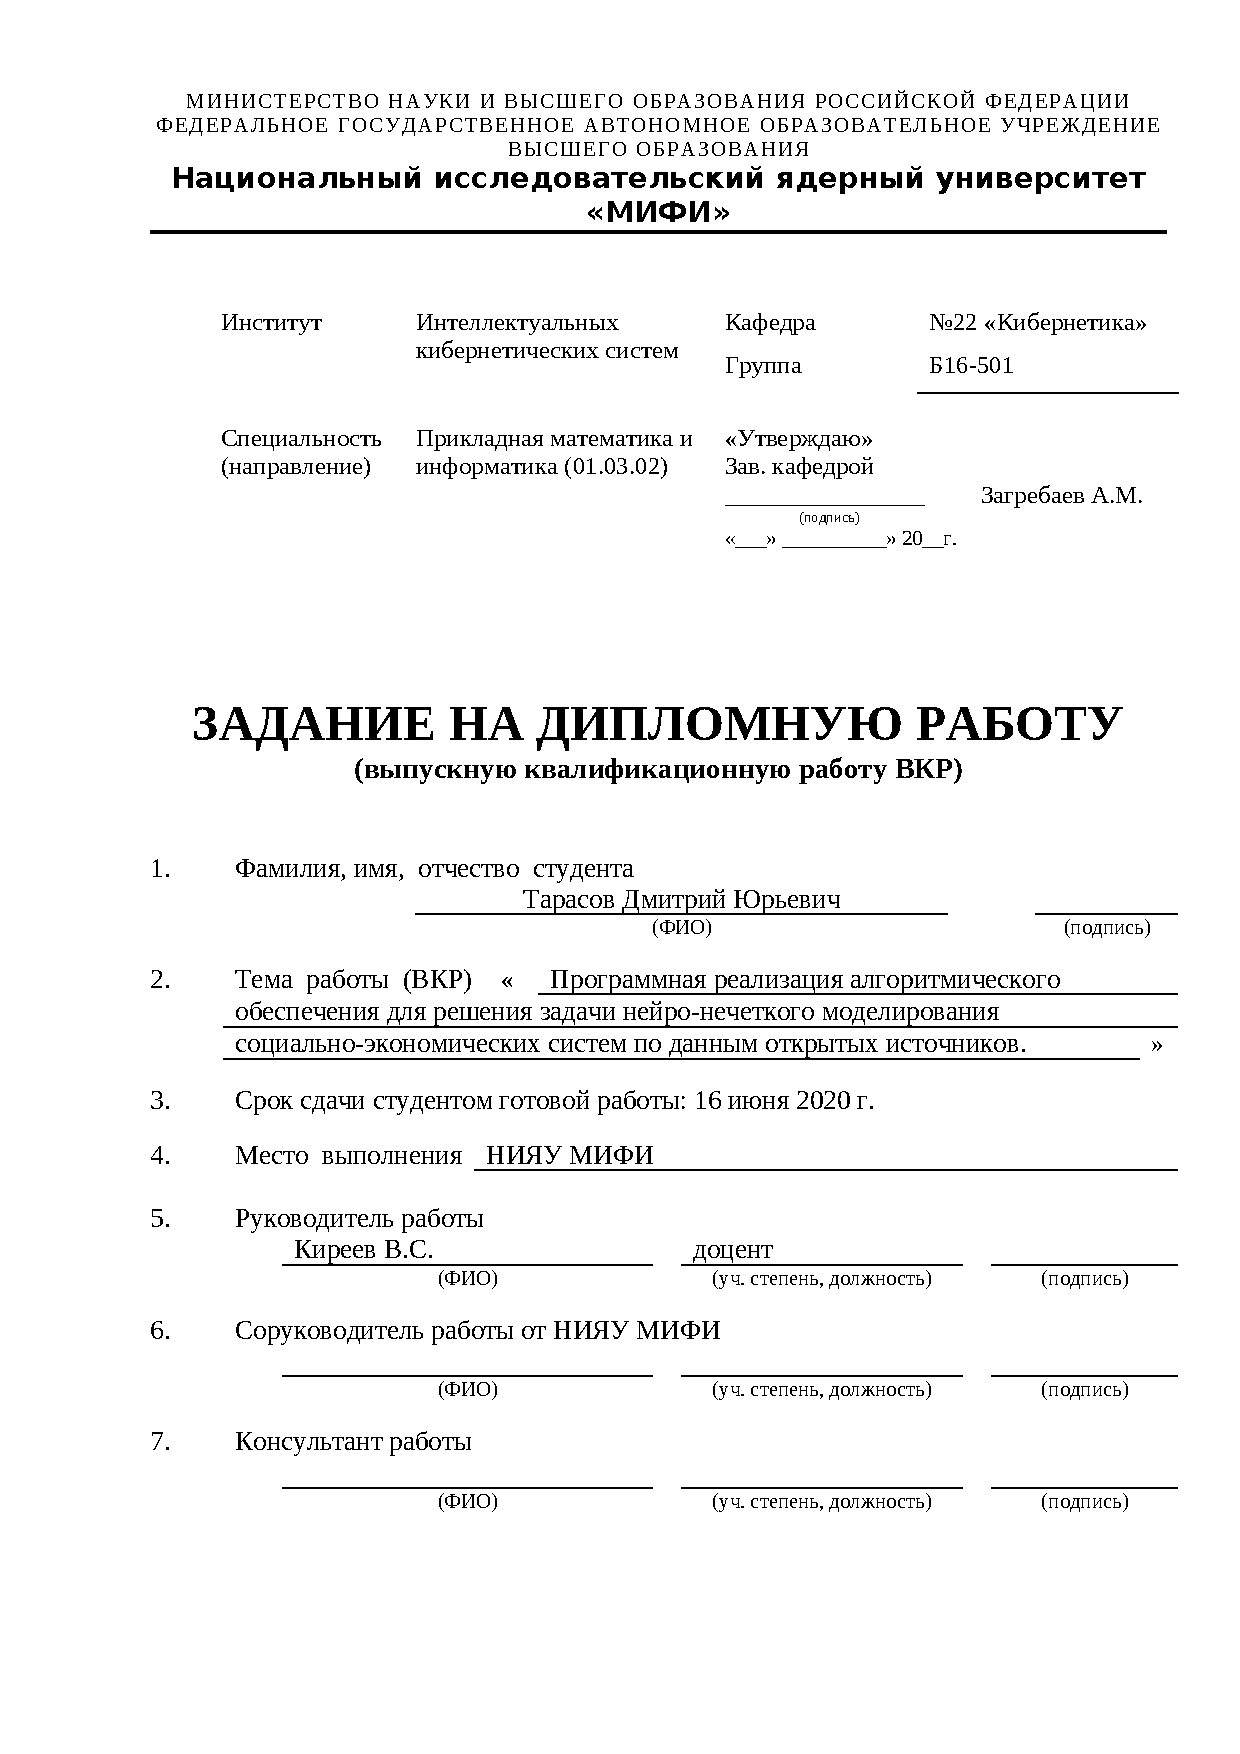
\includepdf[pages={-}, offset=0mm -0mm]{title/task.pdf}


%\clearpage
%\thispagestyle{empty}

%\vfill

%\begin{center}
%[Место для распечатки отчета Антиплагиата]
%\end{center}

%\newpage
%\thispagestyle{empty}

%\vfill

%\begin{center}
%[Место для распечатки отчета Антиплагиата]
%\end{center}

\clearpage

\chapter*{Реферат}
\thispagestyle{plain}

Пояснительная записка содержит N страницы (из них M страниц приложений). Количество использованных источников ~-- M.

Ключевые слова: когнитивные карты, нейро-нечеткие системы,
нейронные сети, LSTM, рекуррентные нейросети, математическое моделирование.

Целью данной работы является создание нечеткой когнитивной карты для моделирования
социально-экономических систем с использованием нейросетевых методов.

В первой главе проводится обзор существующих методов предсказания временных рядов
и модель когнитивных карт.

Во второй главе описываются использованные алгоритмы для оптимизации нечетких
когнитивных карт с помощью нейронных сетей.
Проводится выбор метрик для анализа качества работы алгоритмов.

В третьей главе проектируется архитектура алгоритмического обеспечения
и архитектура модели.

В четвертом разделе проводится функциональное тестирование приложения.


\clearpage

\tableofcontents{}

\clearpage

\chapter*{Введение}
\label{sec:afterwords}
\addcontentsline{toc}{chapter}{Введение}

Моделирование социально-экономической системы может быть использовано для предсказания
некоторых параметров этой системы в будущем.

Для анализа сложных систем, в которых необходимо принимать к сведению не только результат прогнозирования, но и причинно-следственные связи, используются нечеткие когнитивные карты. Однако оригинальный алгоритм работы когнитивных карт можно улучшить, если использовать для оптимизации весов карты нейронные сети. Такие системы называются нейро-нечеткими. Такие системы позволяют снизить нагрузку на экспертов и добиться лучшей точности результата работы системы.

Актуальность данной работы обусловлена тем, что предиктивные модели
могут быть полезны не только для анализа социально-экономической системы, но и для других задач.
Исследование экономической обстановки в регионах может быть интересно в том числе и органам государственной власти.
Кроме того, в работе используются современные методы оптимизации: для оптимизации весов карты используются нейронные сети.

В теоретической части представлена модель нечеткой когнитивной карты с использованием
нейросетей.

В инженерном разделе будут рассмотрены архитектура веб-приложения и методы обработки данных.

В последнем разделе разработанная нейро-нечеткая система будет протестирована.

\clearpage


% Тема:
% Программная реализация алгоритмического обеспечения
% для решения задачи нейро-нечеткого моделирования
% социально-экономических систем по данным открытых источников.

\chapter{Анализ проблематики }
\label{chapter1}

\begin{annotation}
	В данной главе приводится анализ предметной области.
	Проводится сравнительный анализ методов, с помощью которых
	можно решать задачу моделирование сложных систем.
	В конце раздела формулируются цели и задачи работы.
\end{annotation}


\section{Анализ предметной области}

Социально-экономические системы обычно зависят от большого количества параметров.
Эти параметры могут неявно влиять друг на друга. Для описания состояния такой системы
можно использовать временные ряды. Для того, чтобы изучить такую систему, нужно построить ее модель.

Задача моделирования сложных систем ~- это определение возможных параметров
системы и значений этих параметров. После того, как параметры модели были определены,
можно исследовать поведение системы по полученной модели. Одним из возможных
применений полученной модели может быть прогнозирование поведения модели в будущем.
Также модель может помочь проверить гипотезы, которые выдвигают эксперты.
Кроме того, эксперты могут исследовать причинно-следственные связи на основе моделирования.
Важно отметить, что корреляция в данных не всегда означает причинно-следственную связь.
Поэтому для определения причинно-следственных связей нужен эксперт.

Модель социально-экономической системы может быть использована
для прогнозирования будущих значений параметров системы. Прогноз строится на основании
истории одного или нескольких временных рядов, которые соответствуют историческим данным.

\begin{definition}
	(Временной ряд)
	Временным рядом называются последовательно измеренные через некоторые промежутки времени данные.
\end{definition}

Основные явления в эконометрических временных рядах \cite{voron}:
\begin{itemize}
	\item тренды ~= очищенная от случайностей основная тенденция временного ряда
	\item сезонности ~= периодические отклонения от тренда
	\item разладки ~= резкое изменение свойств наблюдаемого ряда
\end{itemize}

Сезонности тоже можно разделить на несколько типов:

\begin{itemize}
	\item аддитивная сезонность
	\item мультипликативная сезонность
\end{itemize}

\def\figurename{Рис}
\begin{figure}[t]%
	\begin{center}
	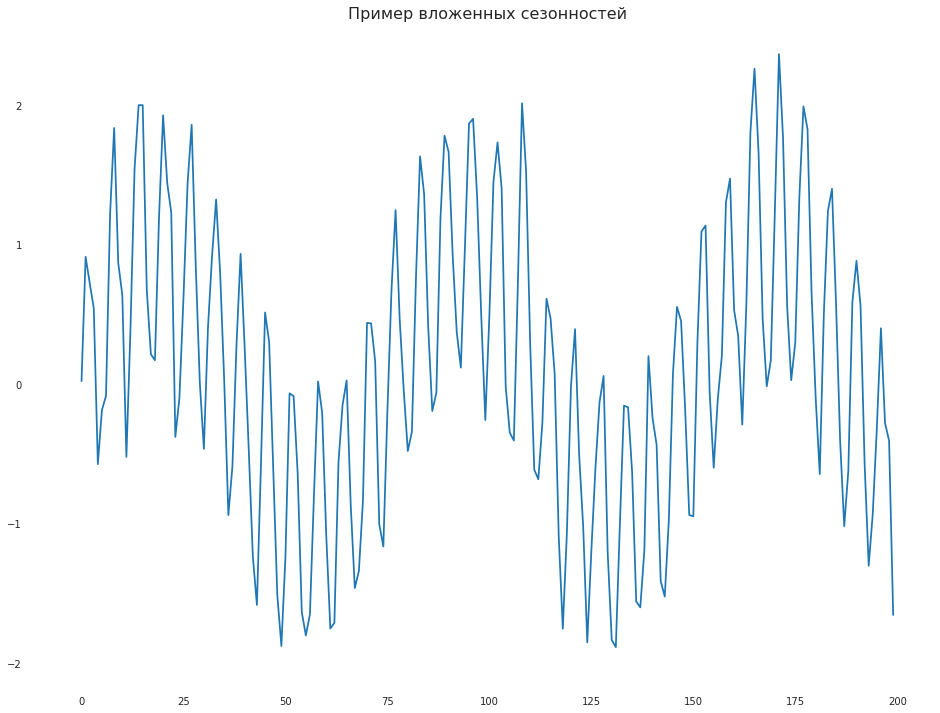
\includegraphics[width=.9\columnwidth]{img/nasted_seasonality.png}%
	\end{center}
	\caption{Пример данных со вложенной сезонностью}%
	\label{img:nasted_seasonality}%
\end{figure}

Кроме того, сезонности могут быть вложенными \ref{img:nasted_seasonality}.
Например, готовая сезонность, месячная, недельная, ежедневная.


Так же при анализе временных рядов нужно учитывать возможные выбросы.
Некоторые временные ряды могут принимать аномальные значения в праздничные дни.
Для таких случаев обычно модель проще обучить реагировать на отдельный входной
параметр, который бы характеризовал о наличии или отсутствии праздников в
определенный день.

Так как в системе может быть много параметров (и, соответственно, временных рядов),
при прогнозировании модель может вычислять будущие значения параметров разными способами:

\begin{itemize}
	\item предсказывать новые значения временного ряда на основе его прошлых значений
	\item предсказывать новые значения временного ряда на основе предыдущих значений
	нескольких параметров, которые могут повлиять на данный параметр
	\item предсказывать сразу несколько временных рядов на основании их предыдущих значений
\end{itemize}

Эти способы перечислены в порядке усложнения модели. Сложность модели влияет на
качество ее предсказаний. Однако выбор слишком сложной модели может повлечь
за собой ее переобучение. Переобучение ведет к тому, что модель теряет способность
к обобщению. Кроме того, сложные модели нужно дольше обучать. И нужно больше данных
для ее качественного обучения. Сложные модели сложнее интерпретировать.

Основные виды моделей для предсказаний временных рядов \cite{voron}:
\begin{itemize}
	\item Aвторегрессионные модели ~= значения временного ряда в данный момент
	линейно зависят от предыдущих значений этого же ряда
	\item Адаптивные модели ~= самонастраивающиеся модели,
	которые способны отражать изменяющиеся во времени условия
	\item Нейросетевые модели
\end{itemize}

% todo адаптивные модели, на самом деле, они являются авторегрессионными?

\section{Сравнительный анализ методов прогнозирования временных рядов}

\textbf{Адаптивные модели} хорошо работают на большом количестве временных рядов.
В случаях, когда необходимо прогноз нужно получить быстро, а учитывать
нужно большое количество факторов. Суть адаптивных
методов заключается в том, что на каждой итерации, после того, как стали
известны новые данные, параметры модели обновляются. Параметры модели вычисляются
на основе исторических данных. Однако такие модели не могут описать сложные
зависимости.

Простота адаптивных методов компенсируется селективными и композиционными моделями.
Можно обучить несколько разных моделей и в зависимости от качества предсказаний на пошедшие
моменты времени для прогнозирования можно использовать ту модель, качество предсказаний
которой выше -~ в этом заключается идея селективных моделей. В композиционных моделях,
результирующим предсказанием выступает взвешенная сумма предсказаний моделей. Вес каждой модели
тоже адаптивный: вычисляются на основании ошибки данной модели.

Обычно адаптивные модели используются для краткосрочного моделирования.
Такие модели при прогнозировании временных рядов учитывают значения только одного временного ряда.
То, что на один временной ряд может влиять значения других временных рядов никак не учитывается.

Преимуществом адаптивных моделей можно считать их простоту и то, что они могут подстраиваться
под изменяющиеся параметры временного ряда.

Простейшим примером адаптивной модели является модель экспоненциального сглаживания \ref{img:exp_smoothing}.
Наблюдения учитываются с убывающими весами.
Чем больше значение $ \alpha $, тем больше сглаживается результат вычислений модели.

\def\figurename{Формула}
\begin{figure}[t]
	\centering
	$ \hat{y_{t+1}} = \alpha y_t + (1 - \alpha)\hat{y_t} $,
	\caption{
		Модель экспоненциального сглаживания.
		$ \alpha $ -~ параметр сглаживания
	}
	\label{img:exp_smoothing}
\end{figure}
\def\figurename{Рис.}


\textbf{Авторегрессионные модели} могут учитывать влияние большого количества параметров
временного ряда. Но чем больше параметров будет иметь модель, тем больше вычислений
потребуется для оценки значений этих параметров.

ARMA -~ модель авторегрессии скользящего среднего. Используется для прогнозирования
стационарных временных рядов.
ARIMA -~ это интегрированная модель авторегрессии. Позволяет объяснить тренд во временном
ряде за счет интегрирования: после того, как посчитаны разности исходного временного ряда,
пелается предположение, что эти разности -~ это стационарный ряд и предсказывается поведение
интегрированного ряда.
ARIMAX -~ модификация ARIMA, в которой в модели регрессии могут учитываться не только предыдущие значения
текущего временного ряда, но и другие экзогенные переменные. Экзогенные переменные могут быть определены
заранее и для прогнозируемого участка временного ряда. Примером экзогенных переменных может служить
индикатор праздников при прогнозировании временных рядов: временной ряд этой экзогенной переменной
будет принимать значение 1 в случае, если в заданных день есть праздник и 0 в других случаях.
SARIMAX -~ ARIMAX с учетом сезонной компоненты. Для учета сезонной компоненты
берутся параметры авторегрессии, интегрирования и скользящего среднего с отставанием
определенным периодом сезонности.

Рассмотрим модель SARIMAX подробнее. Данная модель имеет 7 гиперпараметров:
\begin{itemize}
	\item $ p $ -~ степень авторегрессионной части модели
	\item $ d $ -~ степень интегрирования
	\item $ q $ -~ степень скользящего среднего модели
	\item $ P $ -~ степень авторегрессионной части модели для сезонной компоненты регрессии
	\item $ D $ -~ степень интегрирования для сезонной компоненты регрессии
	\item $ Q $ -~ степень скользящего среднего модели для сезонной компоненты регрессии
	\item $ S $ -~ параметр, определяющий лаг сезонности
\end{itemize}

Также отдельно стоит учитывать экзогенные переменные. Каждая переменная добавляет еще 1 коэффициент
в уравнение регрессии модели.

Определить перечисленные параметры можно перебором различных комбинаций параметров,
или с помощью визуального анализа.

Параметр $ d $ предназначен для того, чтобы избавиться от тренда во временном
ряде. Поэтому график дифференцирования порядка $ d $ должен выглядеть как шум.

Для определения параметра $ p $, следует изучать график частичных автокорреляций.
Если на есть статистически значимые отклонения, то индекс такого отклонения должен соответствовать
значению данного параметра.

Для определения параметра $ q $ необходимо найти статистически значимые отклонения
для автокорреляции ряда.

Важно отметить, что параметры $ p $, $ q $ должны оцениваться для дифференцированного графика.

В \textbf{нейросетевых моделях} тоже можно учесть влияние одного параметра системы на другие.
Суть данных методов похожа на предыдущие: сначала настраиваются начальные
значения параметров модели, а потом эти параметры обновляются, если добавляются новые данные.
Основным отличием можно считать то, что в предсказании одного временного ряда можно
учитывать значения других временных рядов в разные промежутки времени.

Нейросетевые методы можно разделить на 2 вида:
\begin{itemize}
	\item сети прямого распространения
	\item рекуррентные
\end{itemize}

Сети прямого распространения не подразумевают какого-либо состояния.
Поэтому передать информацию о предыдущем шаге итерации можно только явно:
предыдущие значения временного ряда должны передаваться на вход модели.
К сожалению, при таком подходе, количество параметров сети возрастает очень быстро
при увеличении количества предыдущих значений временного ряда. Это сильно усложняет модель,
она легко переобучается. И не может адекватно предсказать новые значения для временного ряда,
потому что теряет способность к обобщению.

Рекуррентные сети наравне с параметрами имеют внутреннее состояние, которое обновляется на каждой
итерации. Это означает, что предсказание будущих значений рядов зависит от "контекста",
то есть от предыдущих вычислений. Данные сети также могут учитывать влияние других
временных рядов на текущий даже с учетом нескольких предыдущих значений.

Но при описании влияния нескольких временных рядов в нейросетевых моделях
нельзя описать, на какой именно ряд влияет другой ряд. Такие знания могут быть у
экспертов. И потенциально, эти знания могли бы упростить модель и уменьшить количество
параметров в ней.

% http://www.machinelearning.ru/wiki/images/archive/c/cb/20160412121749!voron-ml-forecasting-slides.pdf
% todo Как огромное кол-во рядов, после того, как они были предсказаны, потом выливается в предсказание продаж?
% потом просто полносвязной по всем рядам вычисляют значение целевого временного ряда?
% деревья решений?


\section{Описание алгоритма работы нечетких когнитивных карт}

Когнитивная карта – схема причинно-следственных связей в системе.
Когнитивная карта представляет из себя ориентированный граф.
Вершины этого графа – концепты, а ребра – причинно-следственные связи между соответствующими концептами.
Когнитивные карты строятся для того, чтобы понять и проанализировать структуру сложной системы.
Каждое ребро когнитивной карты имеет свой вес, который характеризует степень влияния одного концепта на другой.

Обычно при прогнозировании с использованием нечетких когнитивных карт существует один целевой концепт,
значение которого необходимо спрогнозировать.


Стандартная формула для пересчета значений концептов нечетких когнитивных карт представлена на
\ref{img:concepts_recalc}.

$ A_i(t) $ - значение концепта $A_i$ на шаге $t$.

$ p(x) $ - функция активации \ref{img:sigmiog_actiovation}. Параметр $m$ определяет, на сколько сигмоида будет похожа на пороговую функицю.

\def\figurename{Формула}
\begin{figure}[t]
	\centering
	$ A_j(t+1) = p( A_j(t) + \sum_{i = 1, i \neq j}^{n} w_{ij} A_i(t) ) $,
	\caption{Стандартная формула пересчета значений концептов}
	\label{img:concepts_recalc}
\end{figure}
\noindent

\begin{figure}[t]
	\centering
	$ p(x) = \frac {1} {1+ e^{-mx} } $,
	\caption{Сигмоидальная функция активации}
	\label{img:sigmiog_actiovation}
\end{figure}
\def\figurename{Рис.}

В зависимости от задачи и данных, с которыми работает эксперт могут использоваться и другие
функции активации.

После того, как эксперт построил карту, он может приступить к моделированию поведения
системы и изучением причинно-следственной связи. Таким образом, эксперт может посмотреть,
как изменение одного концепта может повлиять на поведение системы в целом.

Если значения концептов карты расходятся, эксперту нужно или попробовать изменить функцию
активации или изменить значения весов концептов. Возможно, карта несбалансированна из-за
того, что в ней отсутствует еще один компонент, который вносит значительный вклад в поведение системы.

Пересчет значений концептов проходит итеративно. Имея исторические данные эксперт может
подобрать значения весов таким образом, чтобы смоделированное поведение системы как можно меньше отличалось
от экспериментальных данных. В случае классических когнитивных карт эксперту нужно это делать вручную.

После того, как эксперт оптимизировал значения весов, можно приступить к изучению причинно-следственных
связей.

\section{Интеграция когнитивных карт и нейросетей для предсказания временных рядов}

Нейро-нечеткая система - это система, которая включает в себя методы нейронных сетей и методы нечеткой логики.

Поведение объекта в сложных системах прогнозировать непросто.
Часто необходимо знать не только результат прогноза,
но и причинно-следственные связи, которыми был обусловлен данный прогноз
\cite{osoba2019dags} \cite{efficient_fcms}.
Для выявления таких причинно-следственных связей используются нечеткие когнитивные карты.
Следует отметить, что корреляция между временными ряда
Они позволяют качественно оценить влияние разных компонент системы на другие компоненты.
Однако, оригинальный алгоритм для пересчета значений концептов
не может описать сложные зависимости между отдельными компонентами.
Поэтому для того, чтобы увеличить мощность множества зависимостей, которые
может описать модель системы, можно использовать нейросетевые методы.
В таком случае когнитивная карта все еще хранит данные о причинно-следственных связях.

В нейросетевых подходах установить причинно-следственные связи сложнее.
Другие системы, например, деревья решений, наоборот, очень легко интерпретируются, легко обучаются,
но имеют более слабую способность к обобщению.

Идея нечетких когнитивных карт, предложенных Коско \cite{kosko1986fuzzy} имеет следующие преимущества:

\begin{itemize}
	\item Для проведения вычислений требуются небольшие вычислительные мощности.
	\item Простота в использовании.
	\item Можно легко добавлять и удалять концепты.
	\item Можно объединять готовые модели.
\end{itemize}

Однако есть и недостатки:

\begin{itemize}
	\item Веса линейные, нельзя описать сложную зависимость между концептами.
	\item Значение концепта зависит только от значений связанных концептов карты только на предыдущей итерации.
	Невозможно определить связанные во времени концепты больше, чем на одну итерацию.
	\item Веса карты должны быть оценены экспертно.
\end{itemize}

Эти недостатки можно считать существенными.
С этими недостатками можно бороться, если использовать модификации нечетких когнитивных карт,
например, TTR NFCM (Thee Term Relation Neural Fuzzy Cognotive Map) \cite{threeTermNfcm}.

В отличие от классических нечетких карт TTR NFCM позволяет
определять нелинейные функции для весов и при перерасчете значений концептов может учитывать то, как
этот концепт менялся во времени. Возможность использовать нелинейные веса достигается с помощью многослойных прецептронов.
А влияние предыдущих значений концептов определяется размером временного окна, за период которого проводится перерасчет
значений концептов.


\section{Выводы}

\begin{enumerate}
	\item Адаптивные модели хорошо работают на большом количестве временных рядов,
	но не учитывают влияние других рядов на текущий. Они хорошо предсказывают простые зависимости.
	И имеют возможность адаптироваться к новому уровню процесса.
	\item Модификации регрессионных моделей могут позволить описать значительную
	часть информации о временном ряде. Они более интерпретируемы, чем нейросетевые методы, более просты.
	\item Сети прямого распространения плохо подходят для предсказания временных рядов.
	\item Рекуррентные сети хорошо подходят для предсказания временных рядов, но
	с помощью них сложно представить знания о зависимостях между временными рядами.
\end{enumerate}


\section{Постановка задачи работы}


В рассмотренных методах не хватает возможности структурировать экспертные знания.
Для решения этой проблемы могут быть использованы когнитивные карты.
Кроме этого, когнитивные карт разных экспертов можно объединять. Обычно
объединенная карта представляет данные более объективно, потому что возможные
ошибки одного эксперта могут быть компенсированы знаниями другого эксперта.

Целью данной работы является создание нечеткой когнитивной карты для моделирования
социально-экономических систем с использованием авторегрессионных и нейросетевых моделей.

Задачи данной работы:
\begin{itemize}
	\item Разработать алгоритм для интеграции нейросетевых моделей с когнитвными картами.
	\item Сравнить разные модели предсказания временных рядов между собой.
	\item Спроектировать и реализовать модель для когнитивного картирования.
	\item Протестировать полученную модель.
\end{itemize}



\clearpage

\chapter{Разработка моделей и алгоритмов}

% В этой главе описываются разработанные/модифицированные модели/методы/
% алгоритмы, или/и описывается применение известных стандартных методов. Также,
% в конце главы обычно приводится общая архитектура программной системы,
% вытекающая из описанной теории. Приведенные ниже заголовки подразделов так же
% весьма примерные и сильно зависят от особенностей конкретной работы.


\begin{annotation}
	В данной главе описываются алгоритмы работы нечетких когнитивных карт.
	Описывается модифицированная модель когнитивных карт с использованием
	рекуррентных нейросетей и сетей прямого распространения.
	Производится выбор метрик оценки качества работы системы.
\end{annotation}

\section{Описание алгоритма работы нечетких когнитивных карт}

Когнитивная карта – схема причинно-следственных связей в системе.
Когнитивная карта представляет из себя ориентированный граф.
Вершины этого графа – концепты, а ребра – причинно-следственные связи между соответствующими концептами.
Когнитивные карты строятся для того, чтобы понять и проанализировать структуру сложной системы.
Каждое ребро когнитивной карты имеет свой вес, который характеризует степень влияния одного концепта на другой.

Обычно при прогнозировании с использованием нечетких когнитивных карт существует один целевой концепт,
значение которого необходимо спрогнозировать.


Стандартная формула для пересчета значений концептов нечетких когнитивных карт представлена на
\ref{img:concepts_recalc}.

$ A_i(t) $ - значение концепта $A_i$ на шаге $t$.

$ p(x) $ - функция активации \ref{img:sigmiog_actiovation}. Параметр $m$ определяет, на сколько сигмоида будет похожа на пороговую функицю.

\def\figurename{Формула}
\begin{figure}[t]
	\centering
	$ A_j(t+1) = p( A_j(t) + \sum_{i = 1, i \neq j}^{n} w_{ij} A_i(t) ) $,
	\caption{Стандартная формула пересчета значений концептов}
	\label{img:concepts_recalc}
\end{figure}
\noindent

\begin{figure}[t]
	\centering
	$ p(x) = \frac {1} {1+ e^{-mx} } $,
	\caption{Сигмоидальная функция активации}
	\label{img:sigmiog_actiovation}
\end{figure}
\def\figurename{Рис.}

В зависимости от задачи и данных, с которыми работает эксперт могут использоваться и другие
функции активации.

После того, как эксперт построил карту, он может приступить к моделированию поведения
системы и изучением причинно-следственной связи. Таким образом, эксперт может посмотреть,
как изменение одного концепта может повлиять на поведение системы в целом.

Если значения концептов карты расходятся, эксперту нужно или попробовать изменить функцию
активации или изменить значения весов концептов. Возможно, карта несбалансированна из-за
того, что в ней отсутствует еще один компонент, который вносит значительный вклад в поведение системы.

Пересчет значений концептов проходит итеративно. Имея исторические данные эксперт может
подобрать значения весов таким образом, чтобы смоделированное поведение системы как можно меньше отличалось
от экспериментальных данных. В случае классических когнитивных карт эксперту нужно это делать вручную.

После того, как эксперт оптимизировал значения весов, можно приступить к изучению причинно-следственных
связей.

\section{Интеграция когнитивных карт и нейросетей для предсказания временных рядов}

Нейро-нечеткая система - это система, которая включает в себя методы нейронных сетей и методы нечеткой логики.

Поведение объекта в сложных системах прогнозировать непросто.
Часто необходимо знать не только результат прогноза,
но и причинно-следственные связи, которыми был обусловлен данный прогноз
\cite{osoba2019dags} \cite{efficient_fcms}.
Для выявления таких причинно-следственных связей используются нечеткие когнитивные карты.
Они позволяют качественно оценить влияние разных компонент системы на другие компоненты.
Однако, оригинальный алгоритм для пересчета значений концептов
не может описать сложные зависимости между отдельными компонентами.
Поэтому для того, чтобы увеличить мощность множества зависимостей, которые
может описать модель системы, можно использовать нейросетевые методы.
В таком случае когнитивная карта все еще хранит данные о причинно-следственных связях.

В нейросетевых подходах установить причинно-следственные связи сложнее.
Другие системы, например, деревья решений, наоборот, очень легко интерпретируются, легко обучаются,
но имеют более слабую способность к обобщению.

Идея нечетких когнитивных карт, предложенных Коско \cite{kosko1986fuzzy} имеет следующие преимущества:

\begin{itemize}
	\item Для проведения вычислений требуются небольшие вычислительные мощности.
	\item Простота в использовании.
	\item Можно легко добавлять и удалять концепты.
	\item Можно объединять готовые модели.
\end{itemize}

Однако есть и недостатки:

\begin{itemize}
	\item Веса линейные, нельзя описать сложную зависимость между концептами.
	\item Значение концепта зависит только от значений связанных концептов карты только на предыдущей итерации.
	Невозможно определить связанные во времени концепты больше, чем на одну итерацию.
	\item Веса карты должны быть оценены экспертно.
\end{itemize}

Эти недостатки можно считать существенными.
С этими недостатками можно бороться, если использовать модификации нечетких когнитивных карт,
например, TTR NFCM (Thee Term Relation Neural Fuzzy Cognotive Map) \cite{threeTermNfcm}.

В отличие от классических нечетких карт TTR NFCM позволяет
определять нелинейные функции для весов и при перерасчете значений концептов может учитывать то, как
этот концепт менялся во времени. Возможность использовать нелинейные веса достигается с помощью многослойных прецептронов.
А влияние предыдущих значений концептов определяется размером временного окна, за период которого проводится перерасчет
значений концептов.

\section{LSTM NFCM -~ Long Short-Serm Memory Neural Fuzzy Cognotive Map}

Можно усовершенствовать модель TTR LSTM, рассмотренную в предыдущем разделе,
если вместо сетей прямого распространения использовать рекуррентные сети,
например, LSTM \cite{LSTM_paper}. Такая сеть позволит более естественно
сохранять информацию об истории концептов в своем скрытом состоянии,
а для того, чтобы учитывать значения концептов на предыдущих итерациях
в сетях прямого распространения, каждый предыдущий шаг должен быть
описан как отдельная "фича", как отдельный параметр модели.

Сравнение LSTM NFCM с полносвязными сетями:
У LSTM NFCM меньше параметров по сравнению с сетью прямого распространения,
которая бы учитывала больше количество предыдущих значений во временном ряде.
LSTM NFCM дольше обучается, но имеет значительно лучшую способность к предсказанию
на длинных временных рядах.
Модель будет дольше обучаться, потому что нельзя распараллелить
процесс обучения LSTM сетей, так как в сети учитывается, что внутренее состояние меняется последовательно.
LSTM NFCM имеет лучшую интерпретируемость, так как содержит
экспертную информацию о взаимосвязи концептов.
Но для построения LSTM NFCM требуется эксперт, а как следствие,
ручная работа.

Сравнение LSTM NFCM с TTR NFCM:
LSTM NFCM дольше обучается, но на сложных данных
может иметь более точные прогнозы.

Сравнение LSTM NFCM с LSTM:
LSTM сеть, которая бы соответствовала LSTM NFCM, будет иметь
больше параметров в случае, если граф LSTM NFCM не слишком
много связей. LSTM NFCM лучше интерпретируема.
Скорость обучения, при условии оптимизаций в LSTM NFCM, с
помощью которых обучение LSTM моделей в каждой вершине бы проходило
параллельно, будет примерно одинаковой.
Предсказательная способность должна быть лучше у LSTM NFCM.
Потому что такая модель более проста и структурирована.
LSTM модель может оказаться излишне усложненной, так как в ней будет
большое количество параметров.
Но для построения LSTM NFCM требуется эксперт, а как следствие,
ручная работа.
Для построения LSTM NFCM требуется эксперт.

\section{Построение LSTM NFCM}

Для того, чтобы создать модель, нужно определить параметры системы, концепты.
Каждый концепт будет соответствовать вершине графа карты.
После того, как концепты определены, нужно описать взаимодействие между концептами.
Одним из вариантов может быть полносвязный граф, когда каждый концепт имеет
влияние на каждый другой концепт. Теоретически, при увеличении количества
связей в модели, количество возможных зависимостей, которые она может описать
увеличивается. Однако, усложняется и сама модель так, что ее становится сложно обучить.
Слишком сложные модели легко переобучаются на тестовых данных.
Задача эксперта как раз заключается в том, что он должен
описать только необходимые и достаточные взаимосвязи.

Так же, как и большое количество взаимосвязей,
недостаточное количество связей или неверные связи, могут ухудшить
качество модели. Модель может оказаться недостаточно мощной, чтобы описать
исследуемый процесс.

Поэтому важно найти именно существенные связи ме



\section{Алгоритм обучения LSTM NFCM}

% todo нужен рисунок



\section{Алгоритм вычисления LSTM NFCM}

% todo нужен рисунок

\section{Возможные проблемы алгоритма}

Для обучения  нейросети требуется, чтобы
данные для обучения были репрезентативными. То есть
описывали все возможные значения, которые может принимать система.
Во временных рядах, которые представляют

Можно переобучать модель после того, как появляются новые данные.

Если данных очень много (больше тысячи), модель будет потреблять много памяти.
Но данный метод не относится к методам, в которых нужно просто
пользоваться моделью, как молотилкой. А нацелен на то, чтобы наоборот
получить больше понимания о процессе.

При достаточно большом количестве временных рядов,
становится сложно экспертно определить взаимодействие между концептами.
Для задач с большим количеством рядов для исследования, без
модификаций, данный метод не будет эффективен. Так как потребует
большое количество вычислительных ресурсов.
Для таких задач можно использовать, например, градиентный бустинг \ref{friedman2002stochastic}.

\section{Возможные дальнейшие направления для исследований}

Предложенная модель довольно долго обучается и требует много ресурсов
для вычисления. Если найти способ более быстрого вычисления,
теоретически, даже при большом наборе временных рядов, которые нужно
исследовать, можно было бы перебрать различные комбинации взаимосвязей концептов.


\section{Выбор метрик для оценки качества работы алгоритмов}

В качестве критерия качества результата работы системы для предсказаний
для одного временного ряда, можно взять среднеквадратическую
масштабированную ошибку (RMSSE) \ref{hyndman2006another}.
Она вычисляется она по формуле \ref{img:rmsse}

% todo кажется, я это и не использовал
\def\figurename{Формула}
\begin{figure}[t]
	\centering
	$ RMSSE = \sqrt{ \frac{ \frac{1}{h} \sum_{t=n+1}^{n+h}(Y_t - \hat{Y_t})^2  }{ \frac{1}{n-1} \sum_{t=2}^{n} (Y_t - Y_{t-1})^2 } } $,
	$ h --- горизонт предсказаний $,
	$ n --- количество измерений обучающей выборки $,
	$ Y_t --- истинное значение временного ряда в момент времени t $,
	$ \hat{Y_t} --- предсказанное значение временного ряда в момент времени t $,

	\caption{Root Mean Squared Scaled Error}
	\label{img:rmsse}
\end{figure}
\def\figurename{Рис.}

Данная метрика обладает рядом преимуществ:

\begin{itemize}
	\item Ошибка не зависит от масштаба и может быть эффективно использована для предсказаний временных рядов разных масштабов.
	\item Функция может быть вычислена безопасно. Деление на ноль может произойти только если временной ряд состоял из одного повторяющегося числа.
	\item Одинаково штрафуются и положительные, и отрицательные отклонения, метрика симметрична.
\end{itemize}

Для того, чтобы оценить получить ошибку по предсказанию для всех временных рядов,
можно использовать взвешенную среднеквадратическую масштабированную ошибку.
Она вычисляется по формуле \ref{wrmsse}

\def\figurename{Формула}
\begin{figure}[t]
	\centering
	$ WRMSSE = \sum_{i=1}^{k} w_i * RMSSE_i $,
	$ k --- количество временных рядов $,
	$ w_i --- вес ошибки временного ряда i $,
	\caption{Weighted Root Mean Squared Scaled Error}
	\label{img:wrmsse}
\end{figure}
\def\figurename{Рис.}

\section{Выводы}

В данной главе была рассмотрена модель когнитивных карт.
Была разработана модель когнитивных карт
с использованием нейросетей (рекуррентных и прямого распространения).
Были выбраны методы оценки качества работы разрабатываемой системы.

\clearpage

\chapter{Результаты проектирования}

\begin{annotation}
	В данной главе разрабатываются функциональные требования к разрабатываемой системе.
	Проектируется интерфейс модуля. Проектируется структура когнитивной карты.
\end{annotation}


\section{Разработка функциональных требований к системе}

Так как разрабатываемый модуль предназначен для решения задачи, которая
требует интенсивные вычисления, система должна быть реализована
с возможностью оптимизации данных вычислений. Распараллеливать вычисления
можно с помощью видеокарт. Это можно сделать с использованием фреймворка pytorch.

Для проверки качества кода и его работоспособности, должны быть написаны тесты.
Автотесты помогают быстрее находить ошибки и регрессии в функциональности программы.

Эксперт должен иметь возможность задать произвольные концепты, описать
взаимосвязь между концептами явно или неявно, с помощью обученной карты.
Для того, чтобы обучить карту, эксперт должен иметь возможность загрузить
в нее исторические данные.

Эксперт должен иметь возможность построить графики зависимостей концептов
как по историческим данным, так и по предсказанным данным.

Таким образом, функциональные требования:
\begin{itemize}
	\item Возможность распараллеливания вычислений, с использованием фреймворка pytorch.
	\item Система непрерывной интеграции и автоматизированное тестирование.
	\item Поддержка заданных экспертом зависимостей между концептами.
	\item Поддержка зависимостей между концептами, вычисляемых с помощью LSTM.
	\item Возможность визуально представить данные о карте: об истории обучения, качестве модели.
	\item Модуль должен быть расширяемым. Нужна возможность определить пользовательскую функцию для постобработки данных, сгенерированных картой.
	\item Возможность динамических предсказаний. Динамические предсказания --- это
	предсказание, построеное на данных, которые были сгенерированы моделью на предыдущих шагах цикла.
	\item Возможность задать экзогенные параметры через карту.
\end{itemize}

% todo как идея, можно прикрутить мониторинг того, как обучается модель

\section{Архитектура системы непрерывной интеграции}

При отправке новых изменений в исходных текстах модуля,
удаленный репозиторий запускает обработчик тестов.
В этом обработчике запускаются команды, которые
проверяют работоспособность и качество кода в проекте.
В случае ошибок, pull-request блокируется, новые изменения не могут попасть
в ветку $ master $. На почту разработчика приходит уведомление, что
тесты не прошли.

Когда тестов становится слишком много, для того, чтобы было
проще ориентироваться, где именно произошла ошибка,
можно пользоваться отдельными приложениями для построения
отчетов о тестировании. К таким отчетам можно прикреплять
дополнительную отладочную информацию, какую пожелает разработчик тестов.
Однако на данном этапе тестов не будет очень много и это пока что не целесообразно.

\section{Проектирование интерфейса модуля}

Работа с модулем должна состоять из следующих шагов:
\begin{itemize}
	\item Эксперт описывает карту и загружает в нее исходные данные.
	\item Карта обучается.
	\item Выполняется предсказание.
	\item Карта модифицируется, дополняется.
	\item И т д
\end{itemize}

\textbf{Описание концептов.}
При описании карты разработчик может задать
любое количество концептов и связать их любым образом.
При создании концепта требуется указать модель,
по которой будет предсказываться этот концепт, название
концепта и связи концепта с другими концептами.

\textbf{Концепты для автоматического обучения.}
Для автоматического обучения можно использовать LSTM
модель. А также SARIMAX модель для полуавтоматического
обучения. Разработчику будет необходимо задать гиперпараметры
для SARIMAX модели.

\textbf{Концепты для пост-обработки предсказаний.}
Удобно на том же графе, что и строится карта,
иметь возможность задать, как должны быть преобразованы
предсказанные данные. Должна быть возможность
комбинировать разные типы узлов. Также требуется возможность
задавать

\textbf{Обучение.}
Во время обучения, должны быть определены приоритеты
вычислений тех или иных концептов.
Теоретически, этот этап может быть распараллелен.
Все модели, поддерживаемые картой должны
иметь общий интерфейс для обучения и вычисления,
чтобы не нарушать инкапсуляцию. Логика предсказаний
и логика обучения должна быть скрыта внутри модели.

\textbf{Вычисление карты.}
Для вычисления карты от поддерживаемых моделей также требуется
чтобы логика по вычислению моделей не вышла за границы модели.
В зависимости от типа модели должна быть возможность получить
график функции потерь для модели, чтобы оценить качество предсказаний.

\textbf{Модификация карты.}
При добавлении новых концептов, нужно заново обучить
связанные концепты. При удалении концептов, потребуется
переобучение зависимых от удаленного концепта вершин.

\textbf{Моделирование с помощью когнитивной карты.}
Суть моделирования заключается не только в том, чтобы подобрать
оптимальные параметры для выборке для обучения и провалидировать обученную модель.
Эксперт может выдвинуть гипотезу, подстроить параметры модели
и исследовать, как будет вести себя система, анализировать
остатки, которые дает модель. Добавлять или удалять концепты с
целью найти объяснение тем или иным процессам. Так же эксперт
может добавлять в модель экзогенные параметры, которые могут
спрогнозировать поведение системы. Экзогенные параметры
должны быть определены экспертом не только на выборке для обучения,
но и на тестовой выборке. Предполагается, что эти параметры можно вычислить заранее.
В итоге эксперт должен получить граф, который описывает
исследуемый процесс. Этот граф можно интерпретировать
в соответствии с названиями каждой вершины, концепта.
Каждый концепт имеет свою историю значений. И может зависеть или
влиять на другие концепты. Таким образом, он отражает знания
эксперта об исследуемой системе. И с помощью функций, преобразований,
которые эксперт задал на этом графе, может быть получено предсказание
определенных значений концептов.

\textbf{Повторное обучение.}
Так же как и для модификации карты. Не обязательно переобучать всю карту целиком.
Если в этом есть необходимость, можно переобучить только часть карты.


\section{Проектирование структуры когнитивной карты для моделирования количества продаж}

Исследуемые данные представляют из себя несколько временных рядов
за 5 лет по количеству продаж в 3 разных магазинах по 3 разным категориям:

\begin{itemize}
	\item Еда
	\item Товары для дома
	\item Товары для хобби
\end{itemize}

Процесс покупки продуктов --- это социально-экономический процесс.
Количество продаж может зависеть от локальных или национальных праздников.
Продажи по конкретным товарам могут возрастать, если на эти товары есть скидки или акции.
Но так же стоит помнит, что в случае, если товар не завезли,
продажи такого товара будут нулевыми. Но это не значит, что этот товар никому не нужен.

В данной работе будет построена упрощенная модель карты для предсказания количества продаж.
Но влияние экзогенных параметров будет исследовано на других моделях.

Общее количества продаж складывается из сумм продаж
по в каждом магазине:

\begin{equation}\label{eq:sales_total_simple_model}
	STORE\_SALES\_{i} = \sum_{j=1}^{M} CATEGORY\_SALES_{i,j}
\end{equation}

\noindent A продажи в каждом магазине складываются из продаж
товаров каждой категории:

\begin{equation}\label{eq:store_sales_simple_model}
	STORE\_SALES\_{i} = \sum_{j=1}^{M} CATEGORY\_SALES_{i,j}
\end{equation}

Тогда когнитивная карта будет содержать следующие вершины:

\begin{itemize}
	\item $ total\_sales $ --- общее количество продаж
	\item $ store\_id\_TX\_1 $ --- количество продаж в первом магазине
	\item $ store\_id\_TX\_1\_cat\_id\_FOODS $ --- количество продаж в первом магазине в категории "еда"
	\item $ store\_id\_TX\_1\_cat\_id\_HOBBIES $ --- количество продаж в первом магазине в категории "товары для хобби"
	\item $ store\_id\_TX\_1\_cat\_id\_HOUSEHOLD $ --- количество продаж в первом магазине в категории "товары для дома"
	\item $ store\_id\_TX\_2 $ --- количество продаж во втором магазине
	\item $ store\_id\_TX\_2\_cat\_id\_FOODS $ --- количество продаж во втором магазине в категории "еда"
	\item $ store\_id\_TX\_2\_cat\_id\_HOBBIES $ --- количество продаж во втором магазине в категории "товары для хобби"
	\item $ store\_id\_TX\_2\_cat\_id\_HOUSEHOLD $ --- количество продаж во втором магазине в категории "товары для дома"
	\item $ store\_id\_TX\_3 $ --- количество продаж в третьем магазине
	\item $ store\_id\_TX\_3\_cat\_id\_FOODS $     --- количество продаж в третьем магазине в категории "еда"
	\item $ store\_id\_TX\_3\_cat\_id\_HOBBIES $   --- количество продаж в третьем магазине в категории "товары для хобби"
	\item $ store\_id\_TX\_3\_cat\_id\_HOUSEHOLD $ --- количество продаж в третьем магазине в категории "товары для дома"
\end{itemize}

Для моделирования продаж по каждой категории в конкретном магазине
будет использоваться LSTM.
Таким образом имея предсказания продаж для товаров каждой категории в каждом магазине
мы можем явно вычислить количество продаж в магазине целиком и в сумме для трех магазинов.
Для этого необходимо просуммировать результат предсказаний каждой категории
в каждом магазине --- $ CATEGORY\_SALES_{i,j} $.
Для этого при построении карты для значений концептов

\begin{itemize}
	\item $ total\_sales $
	\item $ store\_id\_TX\_1 $
	\item $ store\_id\_TX\_2 $
	\item $ store\_id\_TX\_3 $
\end{itemize}

\noindent будет использоваться простая модель для суммирования.
Особенность ее заключается в том, что модель LSTM в вершинах FCM-LSTM работает
с предыдущими историческими значениями концептов. А модель по суммированию должна работать
с уже предсказанными результатами модели LSTM.

Граф спроектированной карты представлен в приложении \ref{img:fcm_lstm_map}.

\section{Выводы}

В данном разделе были рассмотрена архитектура системы
непрерывной интеграции, выставлены функциональные требования
и спроектирован интерфейс модуля и спроектирована архитектура
когнитивной карты для прогнозирования количества продаж.

\clearpage

\chapter{Реализация и экспериментальная проверка}

\begin{annotation}
	В данной главе приводятся детали разработки и экспериментальной проверки
	разработанной системы. Описан выбор инструментов, используемых для реализации
	программного обеспечения. Приводится выбор инфраструктурных решений,
	с учетом поставленных ранее системных и функциональных требований.
	Описаны состав и структура реализованного программного обеспечения.
\end{annotation}


% todo можно привести таблицу AKAIKE с разными гиперпараметрами для


\section{Выбор инструментальных средств}

В качестве языка программирования для проведения экспериментов и анализа данных
будет использоваться python. Это язык с динамической типизацией, но зато с
большим количеством хорошо протестированных и отлаженых библиотек для работы
с данными (numpy, pandas), статистическим анализом (statmodels) и фреймфорками для построения нейросетей (pytorch, tensorflow).

Для распараллеливания работы с данными и использовании аппаратных ускорений для умножений матриц
для реализации модуля подсистемы обработки данных и подсистемы для вычисления нечеткой карты
будет использоваться pytorch. Это фреймворк для работы с данными и созданию нейросетей.

Конкурентом pytorch является tensorflow, но за счет того, что в pytorch не статический
граф вычислений, а динамический, pytorch предоставляет больше свободы, но и больше мест,
где можно ошибиться.

Недостатком python можно считать динамическую типизацию. Динамическая типизация не позволяет
найти многие ошибки на стадии компиляции. Многие ошибки можно обнаружить только во время
работы программы. Для того, чтобы бороться с этим недостатком, вместе с кодом нужно писать
автоматические тесты --- они позволяют быстро проверить работоспособность программы.

\section{Состав и структура реализованного программного обеспечения}
\begin{annotation}
	В данном разделе рассматривается состав ия структура реализованного программного обеспечения.
	Приводятся характеристики разработанного программного продукта, возможности конфигурации отдельных
	компонент системы. Описано назначение исполняемых файлов, описаны требования к системному окружению.
\end{annotation}

Реализованное по --- это модуль на python, который позволяет помочь эксперту
исследовать моделируемую систему и структурировать знания о системе.

Так как разработка проводилась с методикой Test-Driven-Development,
также были написаны автотесты, которые запускаются
при обновлении кода в удаленном репозитории. Кроме автотестов,
в среде по запуску тестов проверяется качество кода и возможные ошибки
с помощью линтеров на соответствие кода стандарту pep8.
Автотесты необходимы проекту на языке с динамической типизацией,
так как в интерпретируемых языках с динамической типизацией
интерпретатор на стадии компиляции программы не может проверить или вывести, чтобы проверить
типы переменных и аргументов функций самостоятельно. Поэтому код, который
не покрыт тестами может не работать и об этом разработчик узнает
только после того, как программа упадет. Но раннее обнаружение этих
ошибок с помощью автотестов поможет избежать проблем с использованием модуля в
продакшне и поможет сократить время доведения продукта до состояния успешного релиза.

\section{Анализ данных}

Набор данных, на которых будет проводиться тестирование разработанной системы
представляет из себя несколько $ csv $ файлов: файл с количеством продаж
продуктов разных категорий в 3 магазинах за 5 лет начиная с 29.01.2011
и файл с описанием праздников, которые выпадают на каждый день.

Требуется предсказать количество продаж на 30 дней вперед.

Для начала можно провести качественный визуальный анализ данных.

Общее количество продаж можно оценить на графике \ref{img:all_sales}.
Из этого графика видно, что до середины 2012 года количество проданных
товаров увеличивалось. Но после тренд пропал. В данных можно наблюдать
как годичные, так и месячные и даже недельные сезонности. Каждый год
в Рождество количество проданных товаров равно 0, потому что магазин не работает.
По выходным количество проданных товаров больше, чем в будние дни.

Количество проданных товаров по каждому магазину представлено на следующем графике \ref{img:sales_by_store}.
В количестве проданных товаров отдельно по каждому магазину нет значительных отличий.
Все магазины продают примерно одинаковое количество товаров.

Количество продаж по категориям для каждого магазина на графику \ref{img:sales_by_store_by_cat}
Во всех трех магазинах количество продаж товаров в категории "еда" больше всего,
а товаров для дома меньше всего. Из данного графика можно заметить, что сезонность
присутствует в графике по продаже товаров в категории "еда" и для товаров для дома, но
для товаров для хобби сезонности не наблюдаются.

Рассмотрим графики автокорреляции и частичной автокорреляции для общего количества продаж
\ref{img:any_autocorrelation}.
Для лагов 1, 2, 3, 6, 7 присутствует статически значимая частичная автокорреляция.
Это может быть использовано при построении модели SARIMAX.
На графики автокорреляции видны синусоидельные колебания. Это свидетельствует и подтверждает,
что в данных есть сезонность.

\def\figurename{Рис}
\begin{figure}[t]
	\centering
	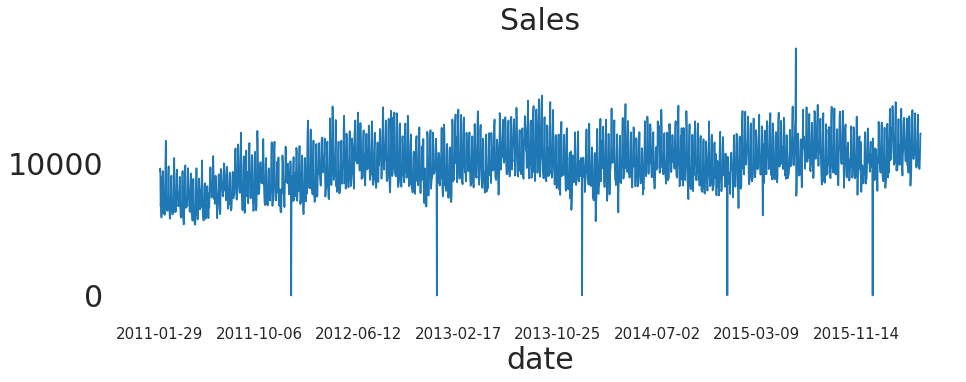
\includegraphics[width=0.9\columnwidth]{./img/all_sales.png}
	\caption{Количество продаж}
	\label{img:all_sales}
\end{figure}


\def\figurename{Рис}
\begin{figure}[t]
	\centering
	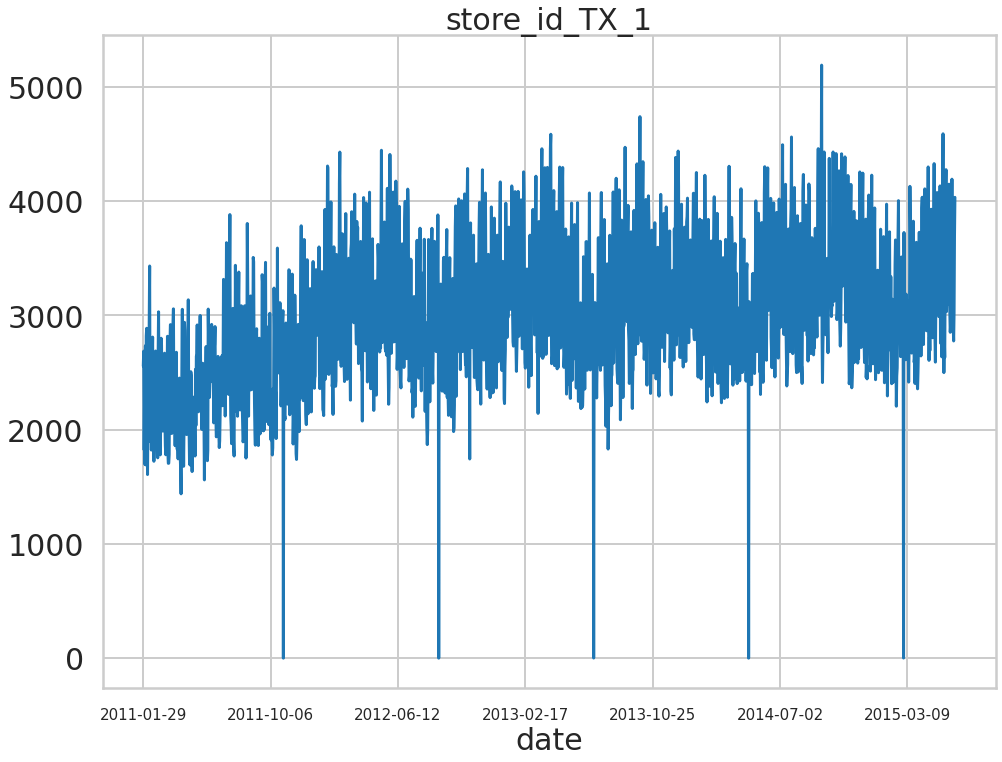
\includegraphics[width=0.25\columnwidth]{./img/store_tx1_total.png}
	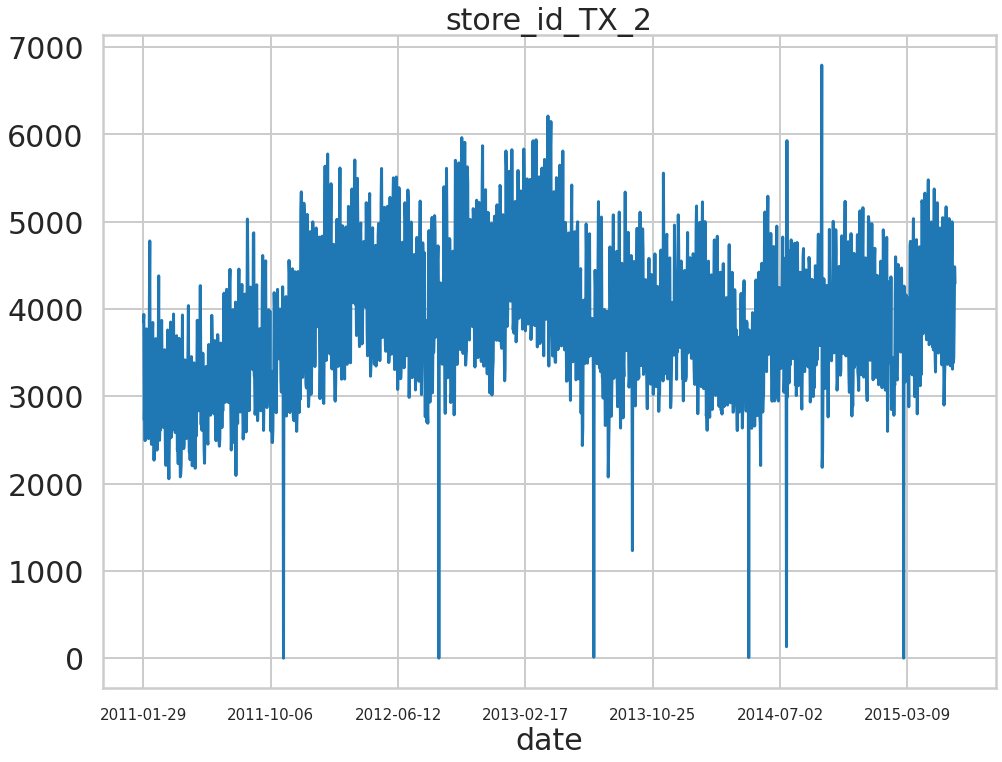
\includegraphics[width=0.25\columnwidth]{./img/store_tx2_total.png}
	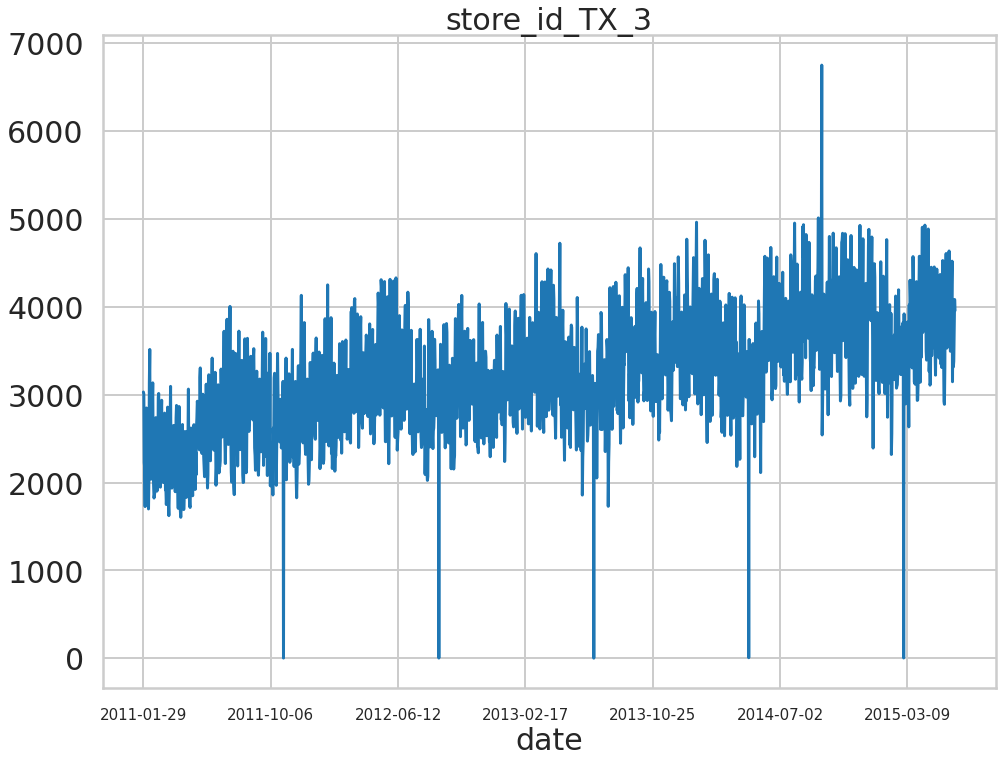
\includegraphics[width=0.25\columnwidth]{./img/store_tx3_total.png}
	\caption{Общее количество продаж по каждому магазину}
	\label{img:sales_by_store}
\end{figure}

\def\figurename{Рис}
\begin{figure}[t]
	\centering
	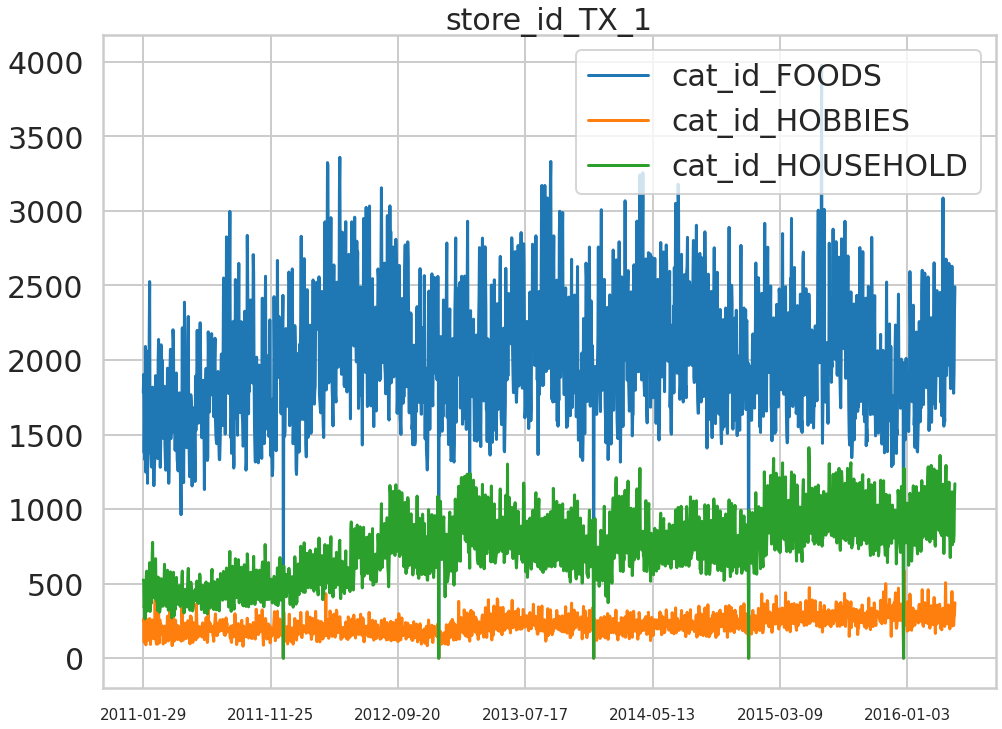
\includegraphics[width=0.25\columnwidth]{./img/store_tx1_by_cats.png}
	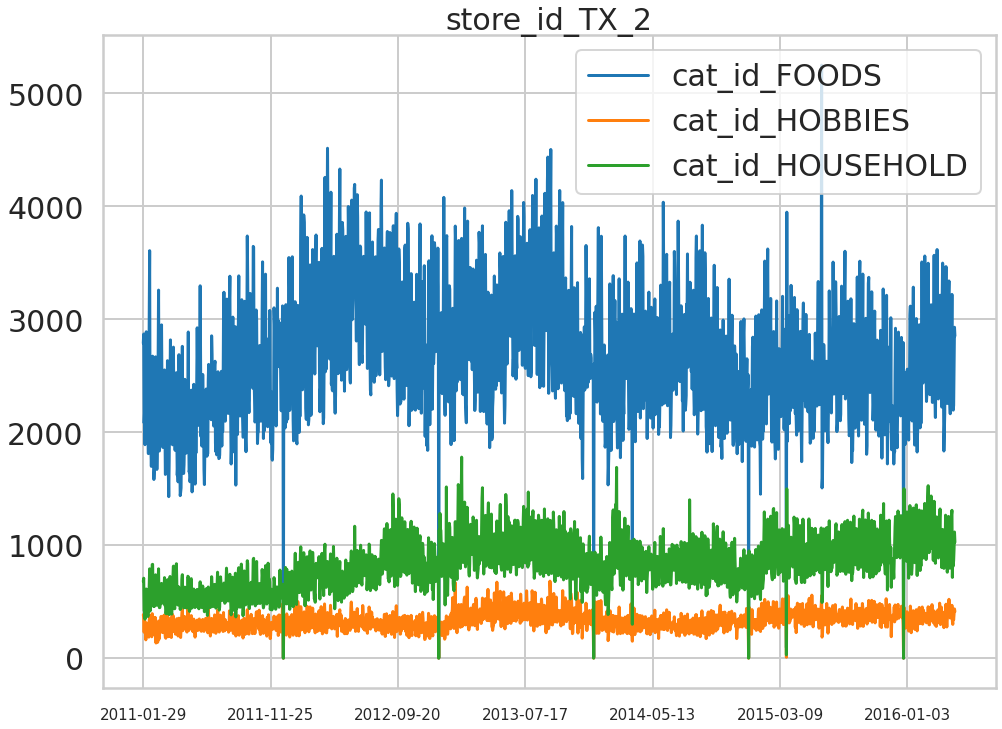
\includegraphics[width=0.25\columnwidth]{./img/store_tx2_by_cats.png}
	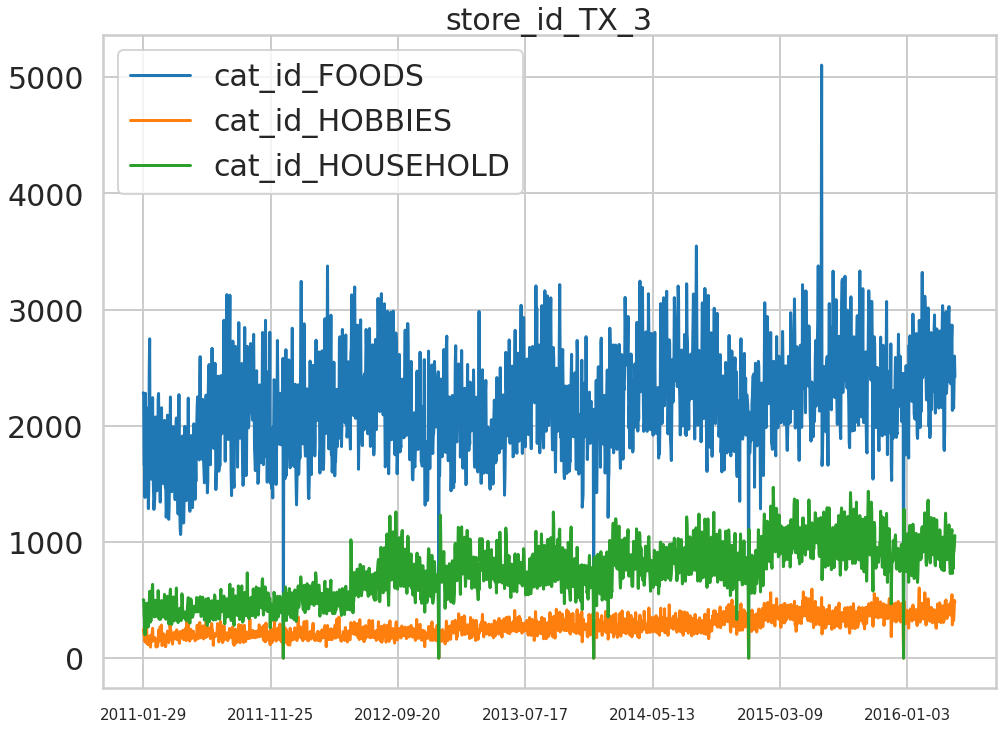
\includegraphics[width=0.25\columnwidth]{./img/store_tx3_by_cats.png}
	\caption{Количество продаж товаров определенной категории для каждого магазина}
	\label{img:sales_by_store_by_cat}
\end{figure}

\def\figurename{Рис}
\begin{figure}[t]
	\centering
	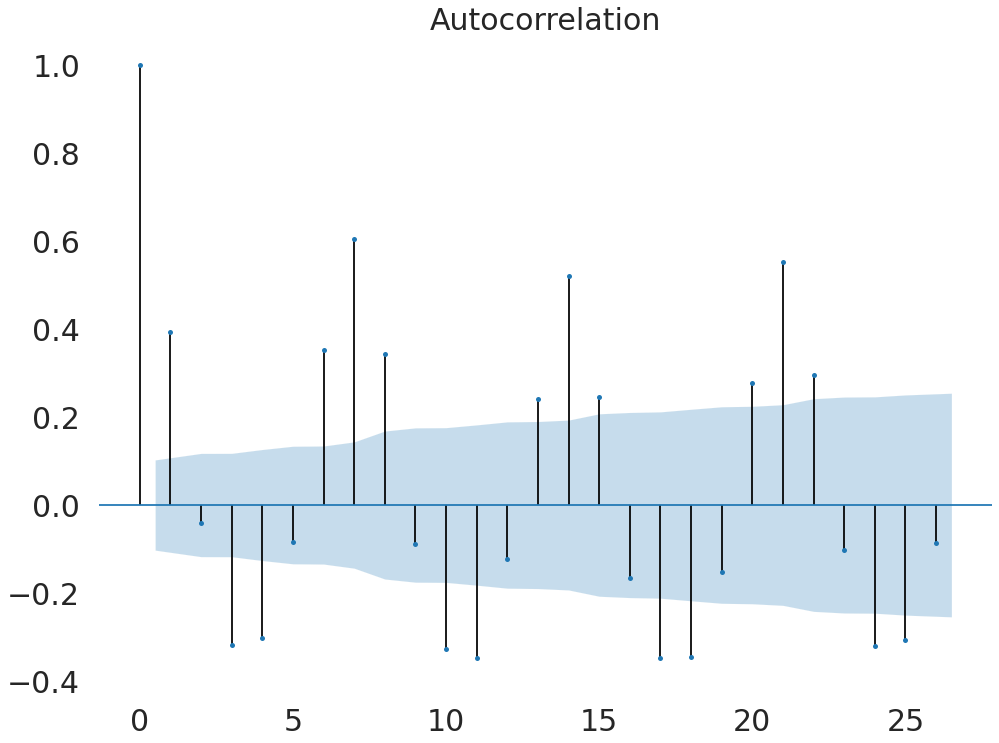
\includegraphics[width=0.4\columnwidth]{./img/sales_autocorrelation.png}
	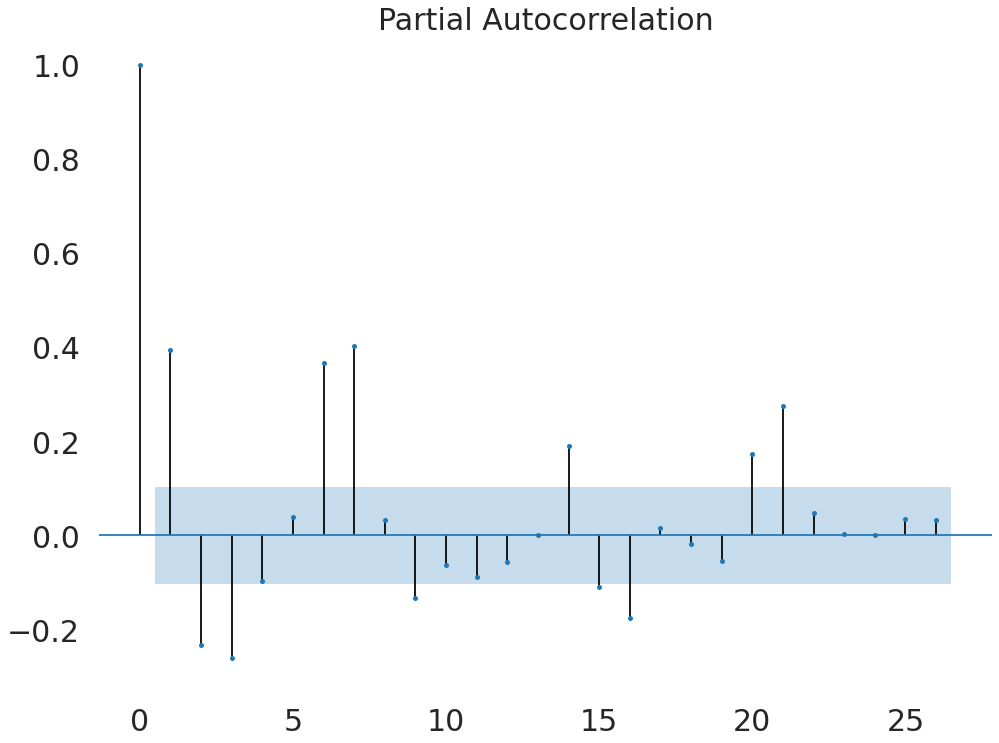
\includegraphics[width=0.4\columnwidth]{./img/sales_partial_autocorrelation.png}
	\caption{Автокорреляция и частичная автокорреляция для общего количества продаж}
	\label{img:any_autocorrelation}
\end{figure}



\section{Построение модели SARIMAX}

Для оптимального подбора гиперпараметров был проведен
визуальный анализ исходных данных, а так же проведена
кросс-валидация с поиском модели с минимальным значением критерия Акаике \cite{akaike}.
Оптимизация параметров на полном наборе данных занимает примерно 10 секунд при 8 параметрах модели.

Оптимальными гиперпараметрами оказались:
$ p = 2, d = 0, q = 3, P = 0, D = 1, Q = 1, S = 7 $.
Сезонность недельная  -~ это логично, что в текущий день
товаров будет продано столько же, как неделю назад.

На графике остатков \ref{img:arimax_resid} все еще прослеживается
годичная сезонность и выбросы. Выбросы -~ предсказать возможно, если
добавить экзогенные параметры в виде индикатора праздников.

В качестве экзогенных параметров рассмотрим индикатор дня недели.
В исходные данные добавится 7 колонок. Каждому дню недели
будет соответствовать одна колонка. И еще одним экзогенным параметром
возьмем индикатор праздника -- Рождества.
Экзогенные параметры можно вычислить заранее, так как наперед можем
поставить в соответствие индикатор дня недели определенному календарному дню
и индикатор Рождества.
Оптимизация параметров модели с 8 экзогенными переменными потребовало 20 секунд.

На графике остатков модели с экзогенными переменными \ref{img:arimax_resid} видно, что удалось избавиться
от большого значения остатков на Рождество. Это получилось сделать благодаря
столбцу-индикатору Рождественских праздников.

\def\figurename{Рис}
\begin{figure}[t]
	\centering
	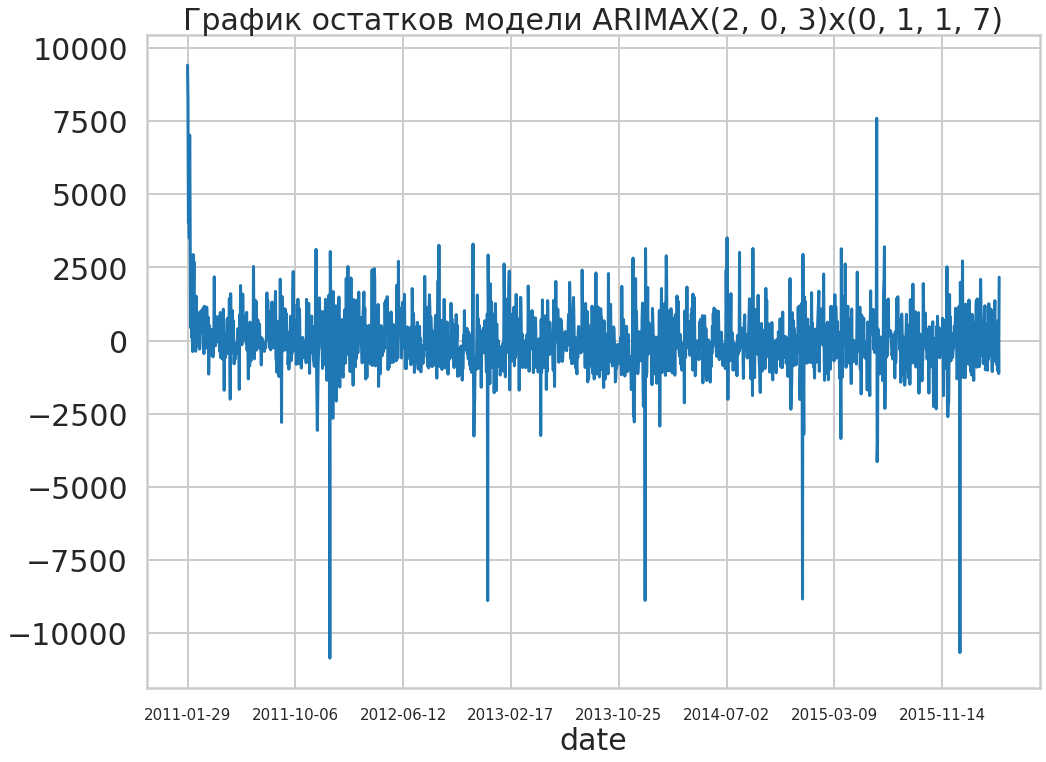
\includegraphics[width=0.4\columnwidth]{./img/arimax_resid.png}
	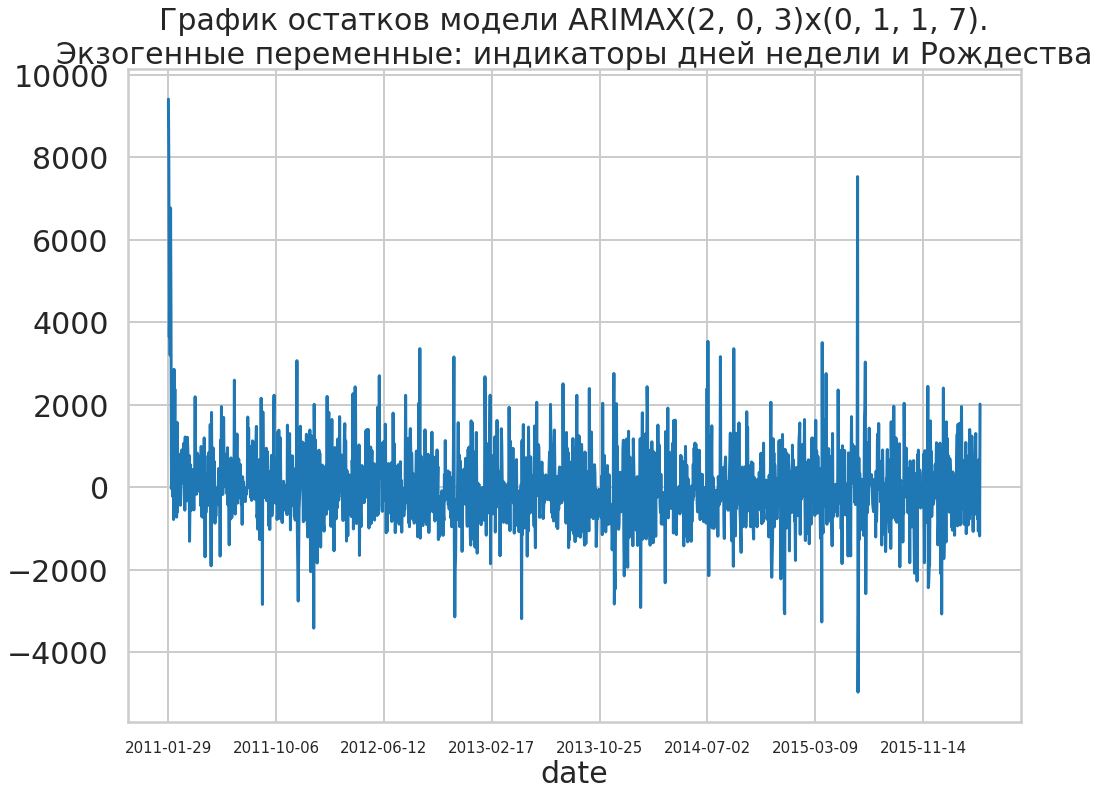
\includegraphics[width=0.4\columnwidth]{./img/arimax_resid_with_xmas.png}
	\caption{График остатков модели ARIMAX с соответствующими параметрами}
	\label{img:arimax_resid}
\end{figure}

Но если проанализировать значения коэффициентов обученной модели \ref{tbl:arimax_coeffs_exogen},
можно заметить, что индикаторы дня недели слишком слабо влияют на предсказание модели.
Значения коэффициентов очень маленькие, вероятность того, что эти параметры будут иметь
значение больше критического равно единице, дисперсия большая. Из этого можно сделать вывод,
что использование этих экзогенных переменных неоправданно. Но зато значение коэффициента
для индикатора Рождества ($ xmas $) большое. Этот экзогенный параметр
действительно объясняет некоторую полезную часть данных. Так, значение теста Харке-Бера
для предыдущей модели было равно $ 37658.88 $, а после выявления зависимости между количеством продаж
и днем рождества стало равно $ 1488.02 $. Чем ближе значение этого теста к нулю, тем больше остатки
модели похожи на нормальное распределение. Этот тест сверяет асимметрию и эксцесс остатков с
значениями этих моментов для нормального распределения. И хотя с таким абсолютным значением
теста нельзя говорить о том, что остатки распределены нормально, но относительно предыдущей
модели, новая модель определенно лучше.

Но на предсказании на 30 дней вперед найденные экзогенные переменные не повлияли \ref{img:arimax_forecast},
так как в исследуемый момент времени не было Рождества.

\def\figurename{Рис}
\begin{figure}[t]
	\centering
	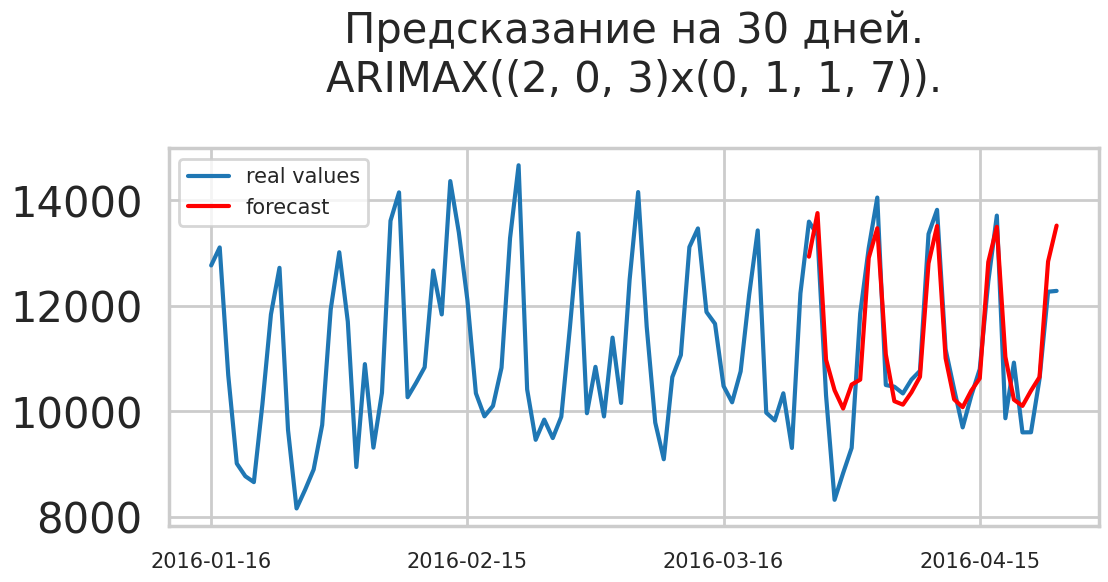
\includegraphics[width=0.9\columnwidth]{./img/arimax_simple_pred30.png}
	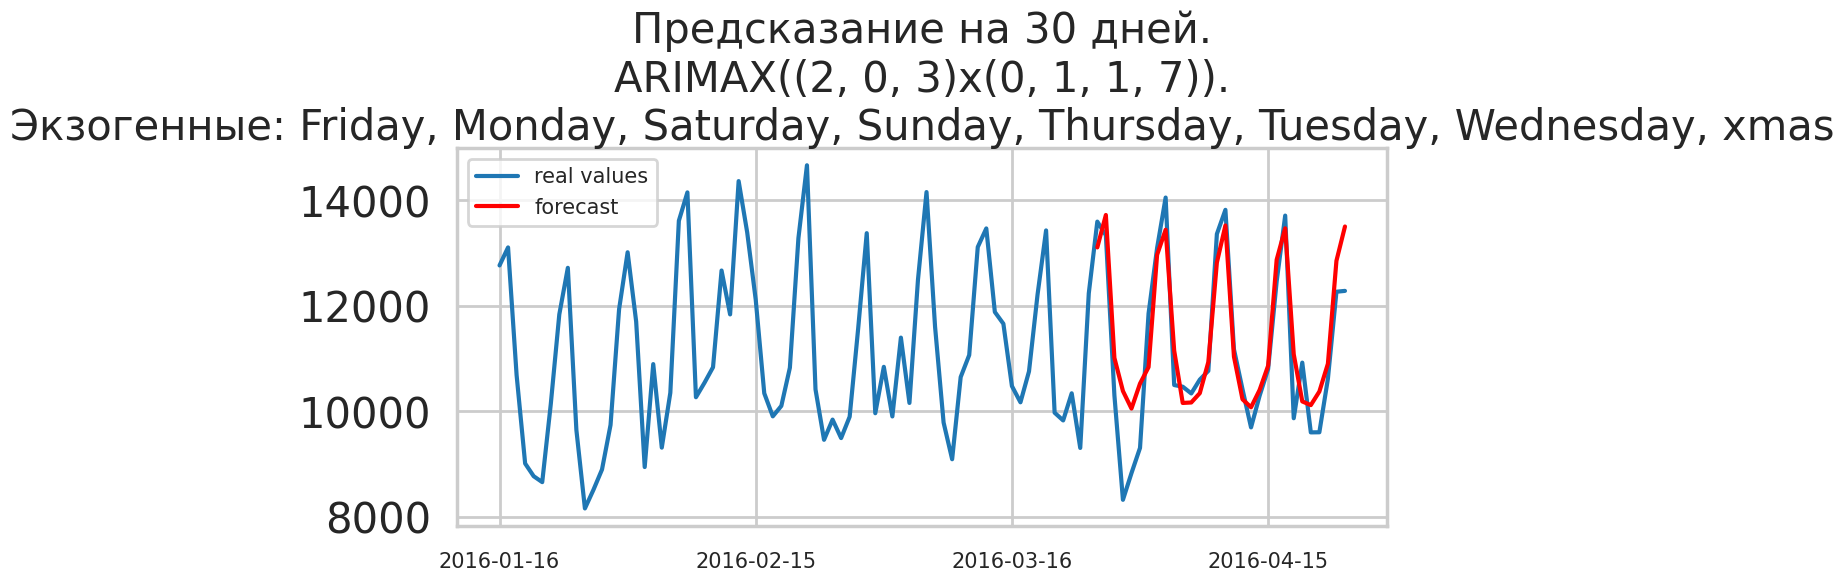
\includegraphics[width=0.9\columnwidth]{./img/arimax_with_exog_pred30.png}
	\caption{Предсказания на 30 дней вперед}
	\label{img:arimax_forecast}
\end{figure}

Значение $ RMSSE $ для модели с экзогенными параметрами ($ RMSSE = 0.000210 $) незначительно меньше
модели без экзогенных переменных ($ RMSSE = 0.000208 $).


\section{Построение модели LSTM}

В отличие от таких статистических методов как ARIMAX, предсказание данных
с помощью нейросетей требует более тщательно предобработки данных.
Перед тем, как скормить данные на вход нейросети, их нужно нормализовать.
Для того, чтобы нормализовать данные, вычтем из данных за каждый день средннее
количество продаж и разделим на стандартное отклонение. После того, как
нейросетевая модель посчитает предсказание, полученные в предсказании
числа нужно будет умножить на стандартное отклонение и прибавить среднее.
Важно, чтобы обучающая выборка была репрезентативной. Так как модель
может вести себя неадекватно, если входные данные слишком сильно отличаются
от данных, которые были на обучающей выборке.

К сожалению, предсказания, которые мы получили с помощью  LSTM менее интерпретируемы,
чем те, которые мы получили с помощью SARIMAX. Однако LSTM --- это намного более
мощная модель. И может быть использована в тех случаях, если мощности SARIMAX не хватает.
Также можно использовать эти модели вместе. Например, сначала с помощью SARIMAX создать
модель, которую можно интерпретировать, а потом с помощью LSTM можно предсказывать остатки, которые будет
давать SARIMAX. И эти остатки можно прибавлять к исходному предсказанию SARIMAX. Такой алгоритм
не позволит повысить интерпретируемость предсказания, но позволит увеличить его точность.
Другой вариант --- это использовать не остатки предсказаний ARIMAX модели, а
сами предсказания в качестве одного из параметров LSTM модели \ref{img:lstm_with_arima_forecast}.
Теоретически, это должно позволить LSTM сети быстрее обучиться.
В результате эксперимента было замечено, что действительно качество предсказаний
на малых итерациях при использовании предсказаний ARIMAX модели в LSTM модели
позволили быстрее получить качественных результат. Но при увеличении количества итераций
получить лучший результат по сравнению с использованием чистой LSTM модели не удалось.
$ RMSSE = 0.000174 $ --- это даже больше, хотя и незначительно, чем у обычной LSTM.

\def\figurename{Рис}
\begin{figure}[t]
	\centering
	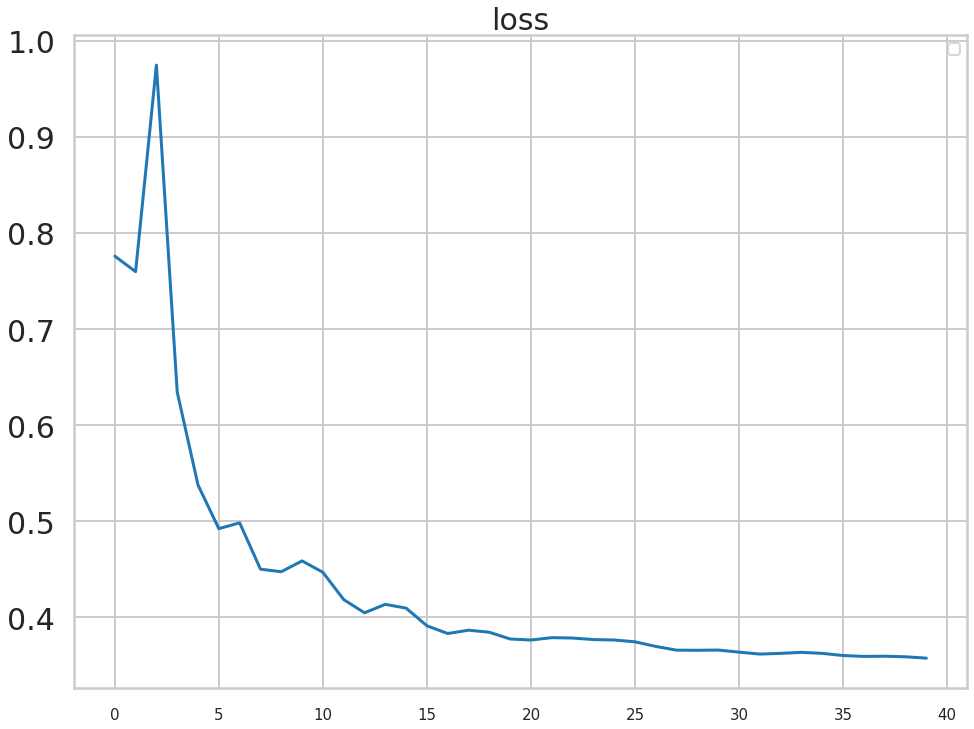
\includegraphics[width=0.4\columnwidth]{./img/lstm_with_arima_loss.png}
	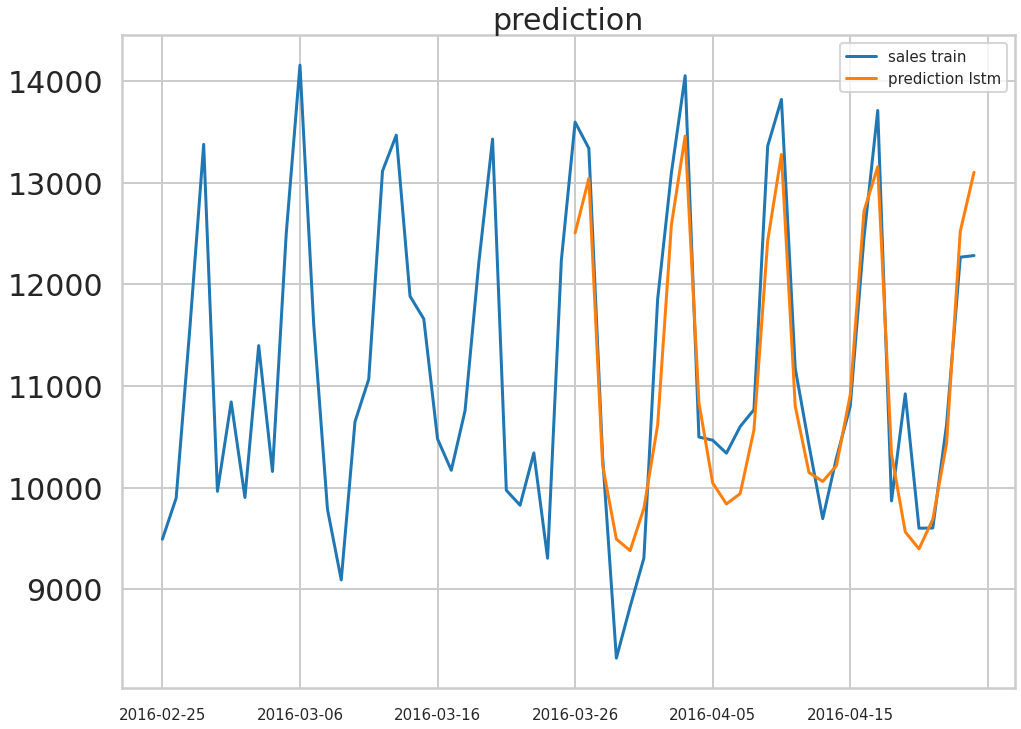
\includegraphics[width=0.4\columnwidth]{./img/lstm_with_arima_prediction.png}
	\caption{Кривая потерь и предсказание LSTM-сети c использованием результатов предсказаний ARIMAX модели}
	\label{img:lstm_with_arima_forecast}
\end{figure}

Результаты предсказаний с помощью модели LSTM очень похожи на результаты предсказаний
с помощью SARIMAX. Стоит заметить, что LSTM была обучена и вычислялась с помощью GPU.
В то время как оптимизация параметров модели SARIMAX производились на процессоре и
для получения примерно одинаковых результатов требовалось столько же времени.
Если бы LSTM обучалась на процессоре, время обучения бы исчислялось не секундами, а часами,
так как это затратный по вычислительным мощностям процесс.

В результате эксперимента была обучена LSTM сеть с размерностью скрытого слоя равной 200.
Результат обработки LSTM-сети после ее вычислений попадал в полносвязную сеть с размерностью
тоже 200. Кривая потерь в процессе обучения и график с предсказаниями представлены не графиках \ref{img:lstm_forecast}.
Значение $ RMSSE = 0.000167 $. Это немного меньше, чем у модели SARIMAX, но незначительно.

Кроме того, важным недостатком такой модели может быть то, что она не
способна предсказывать новые данные, например, линейную зависимость.
Для того, чтобы предсказать временной ряд с трендом, нужно или делать
декомпозицию или преобразовать исходный ряд так, чтобы в нем не было тренда.
После того, как получили предсказания, нужно проделать обратные преобразования.
Это не всегда удобно.

\def\figurename{Рис}
\begin{figure}[t]
	\centering
	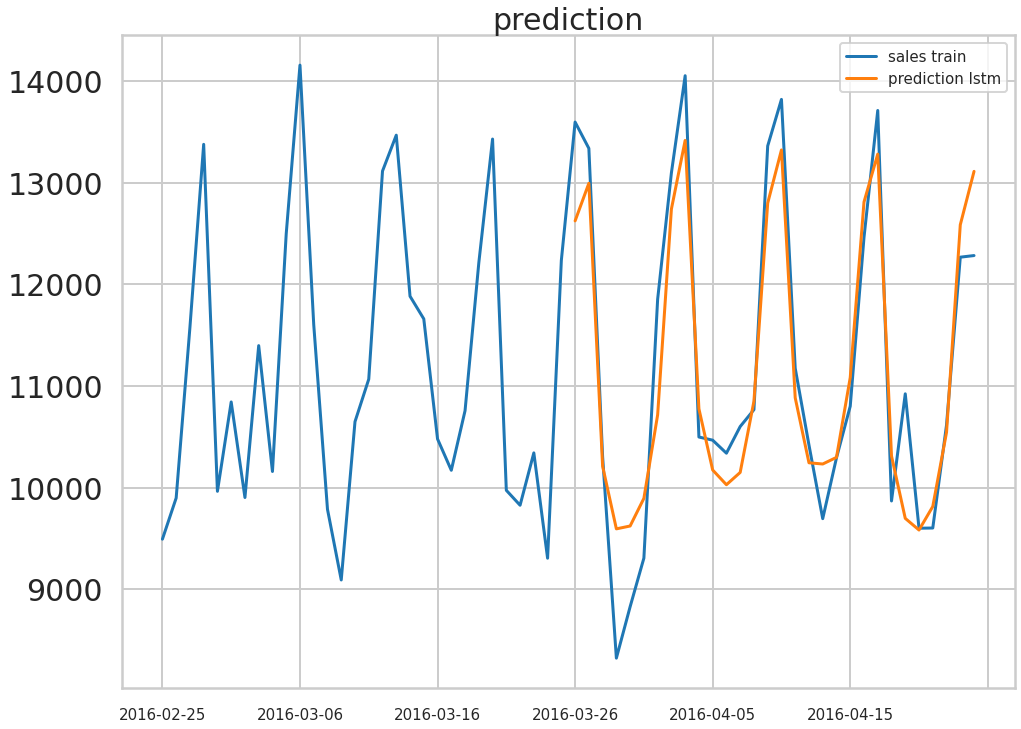
\includegraphics[width=0.4\columnwidth]{./img/lstm_prediction.png}
	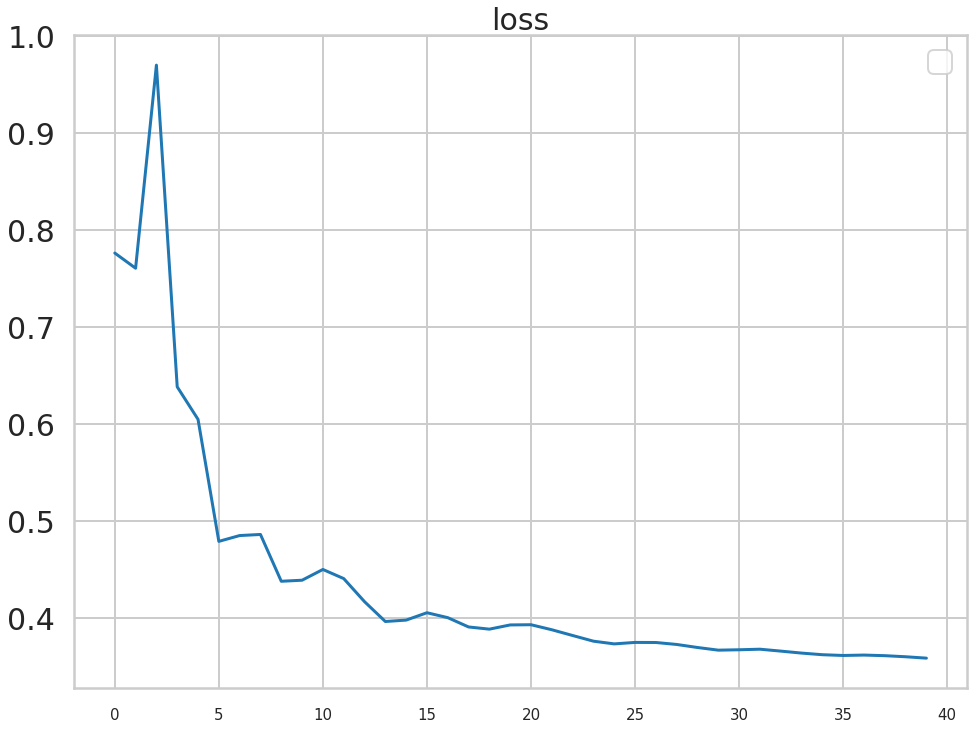
\includegraphics[width=0.4\columnwidth]{./img/lstm_loss.png}
	\caption{Кривая потерь и предсказание LSTM-сети}
	\label{img:lstm_forecast}
\end{figure}

\section{Построение модели FCM}


% \section{Тестирование разработанной системы}

% Для тестирования системы были построены 3 варианта карты:
% \begin{itemize}
% 	\item Карта без связей.
% 	\item Полносвязная карта.
% 	\item Карта с осмысленными связями.
% \end{itemize}

% Все карты обучались 100 эпох, имели размерность скрытого состояния 100,
% количество исторических данных, обрабатываемых с помощью LSTM на одной итерации -~ 100.
% Так же как и количество данных на выходе, сгенерированных.

% Карта без связей \ref{img:lstmfcm_empty}, обученная на тестовых данных
% показала отличный результат для $ x_1, x_2, x_3, x_4  $. Однако ошибка
% для $ x_5, y $ довольно велика. Такие предсказания эквивалентны предсказаниям
% отдельно взятых моделей LSTM, обученных для предсказания временного ряда
% по истории только этого временного ряда.

% Карта, которая представляет из себя полносвязный граф \ref{img:lstmfcm_fc},
% из-за избыточности связи получила предсказания для $ x_1, x_2, x_3 $ даже
% хуже, чем карта без связей. Это можно объяснить излишней сложностью модели.
% Модель слишком усложнена и не может обучиться за заданное количество эпох.

% Карте с осмысленными связями \ref{img:lstmfcm_meaningful} удалось сохранить качество
% предсказаний для $ x_1 --- x_4 $ таким же, как и у карты без связей.
% А так же удалось получить улучшение предсказания для $ y $.
% Неожиданный результат получили для $ x_5 $. todo как так?

% Для карт, у которых были связи с $ x_5, y $ получилось лучше предсказать значения
% для этих рядов. Потому что значения этих рядов зависят от $ x_1 --- x_4 $.

% Кроме того, на долгосрочных предсказаниях видно, что $ x_4 $ имеет проседания.
% Вероятно, это связано с ограничениями, рассмотренными во второй главе.
% Так как модель обучается на одних данных, а после предсказания, модель возвращает
% данные в новой области значений, будущие предсказания становятся все более нестабильными.
% todo не понятно, почему их нет на предсказании LSTM

% \def\figurename{Рис}
% \begin{figure}[t]
% 	\centering
% 	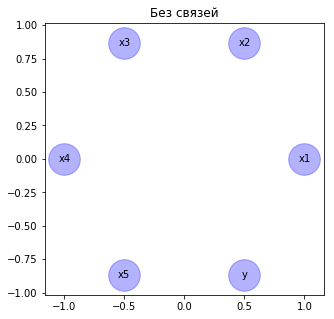
\includegraphics[width=0.7\columnwidth]{./img/lstmfcm_empty.png}
% 	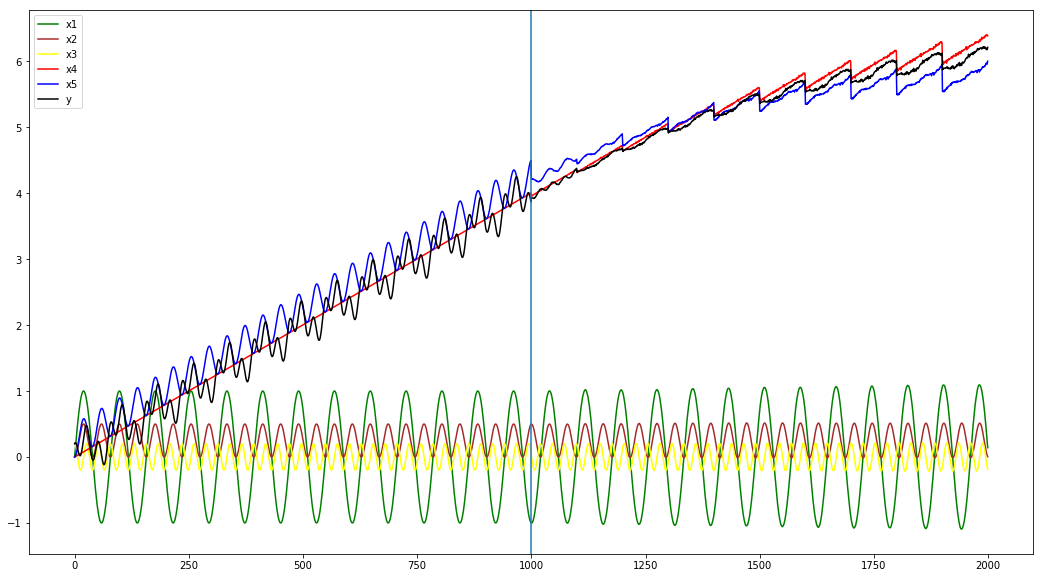
\includegraphics[width=0.9\columnwidth]{./img/lstmfcm_empty_prediction.png}
% 	\caption{Карта без связей концептов}
% 	\label{img:lstmfcm_empty}
% \end{figure}

% \begin{figure}[t]
% 	\centering
% 	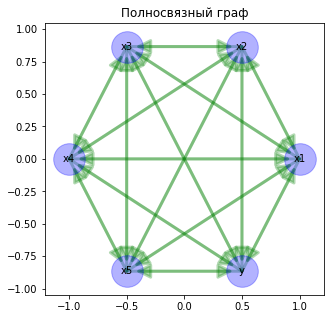
\includegraphics[width=0.7\columnwidth]{./img/lstmfcm_fc.png}
% 	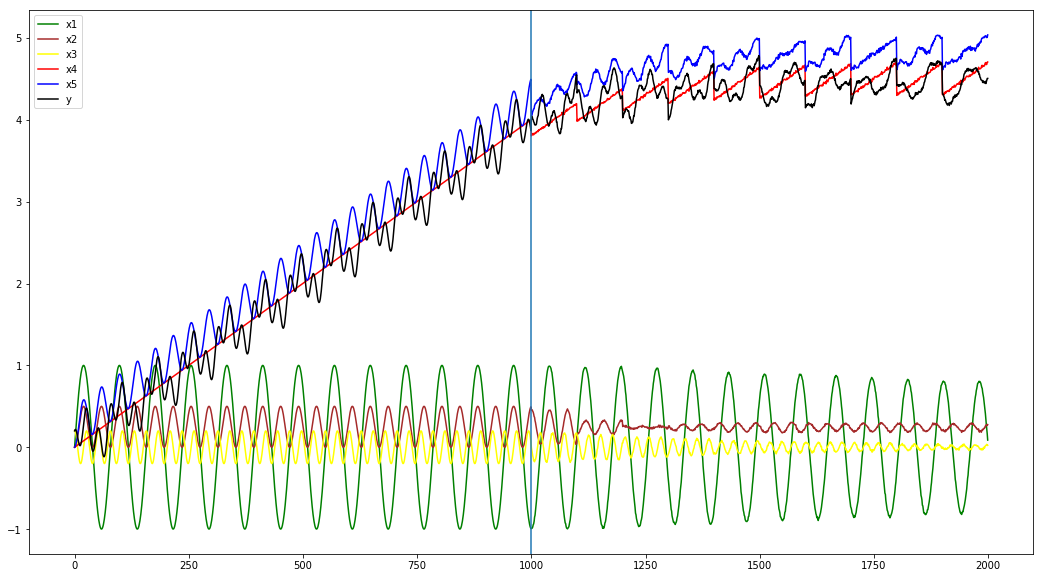
\includegraphics[width=0.9\columnwidth]{./img/lstmfcm_fc_prediction.png}
% 	\caption{Полносвязная карта}
% 	\label{img:lstmfcm_fc}
% \end{figure}

% \begin{figure}[t]
% 	\centering
% 	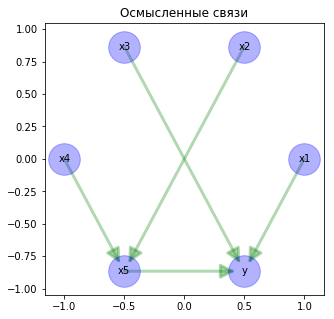
\includegraphics[width=0.7\textwidth]{./img/lstmfcm_meaningful.png}
% 	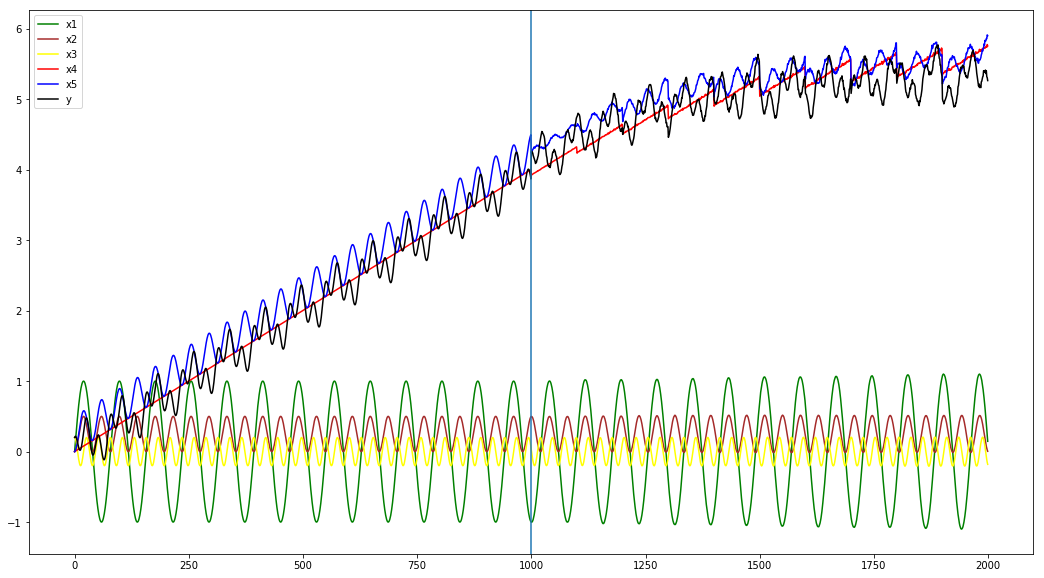
\includegraphics[width=0.9\textwidth]{./img/lstmfcm_meaningful_prediction.png}
% 	\caption{Карта с осмысленно расставленными связями}
% 	\label{img:lstmfcm_meaningful}
% \end{figure}


% \section{Экспериментальное сравнение разработанной системы с существующими}

% Была построена модель, основанная на LSTM,
% которая одновременно анализирует все временные ряды тестовых данных.

% Результат предсказаний такой модели представлен на рисунке \ref{img:lstm_only_prediction}.
% Результат зашумлен по сравнению с предсказаниями карты (todo не могу объяснить).
% И в отличие от карты, даже с осмысленными связями, на этом предсказании не наблюдается скачков
% между итерациями предсказаний. И $ x_5 $ тоже удалось предсказать относительно успешно.

% Данная модель так же, как и карта работала рекурсивно:
% на каждой следующей итерации обрабатывала данные, полученные на предыдущей.
% Скачок вначале предсказаний, скорее всего, связан с тем, что после обучения,
% скрытое состояние сети выставляется заново, так как меняется его размерность.
% Возможно, использование скрытого состояния одинаковой размерности во время
% тренировки и во время тестирования, может избавить от этой проблемы. Однако
% в LSTM NFCM между итерациями тоже сохраняются эти скачки, хотя между итерациями
% скрытое состояние не переинициализируется.

% \begin{figure}[t]
% 	\centering
% 	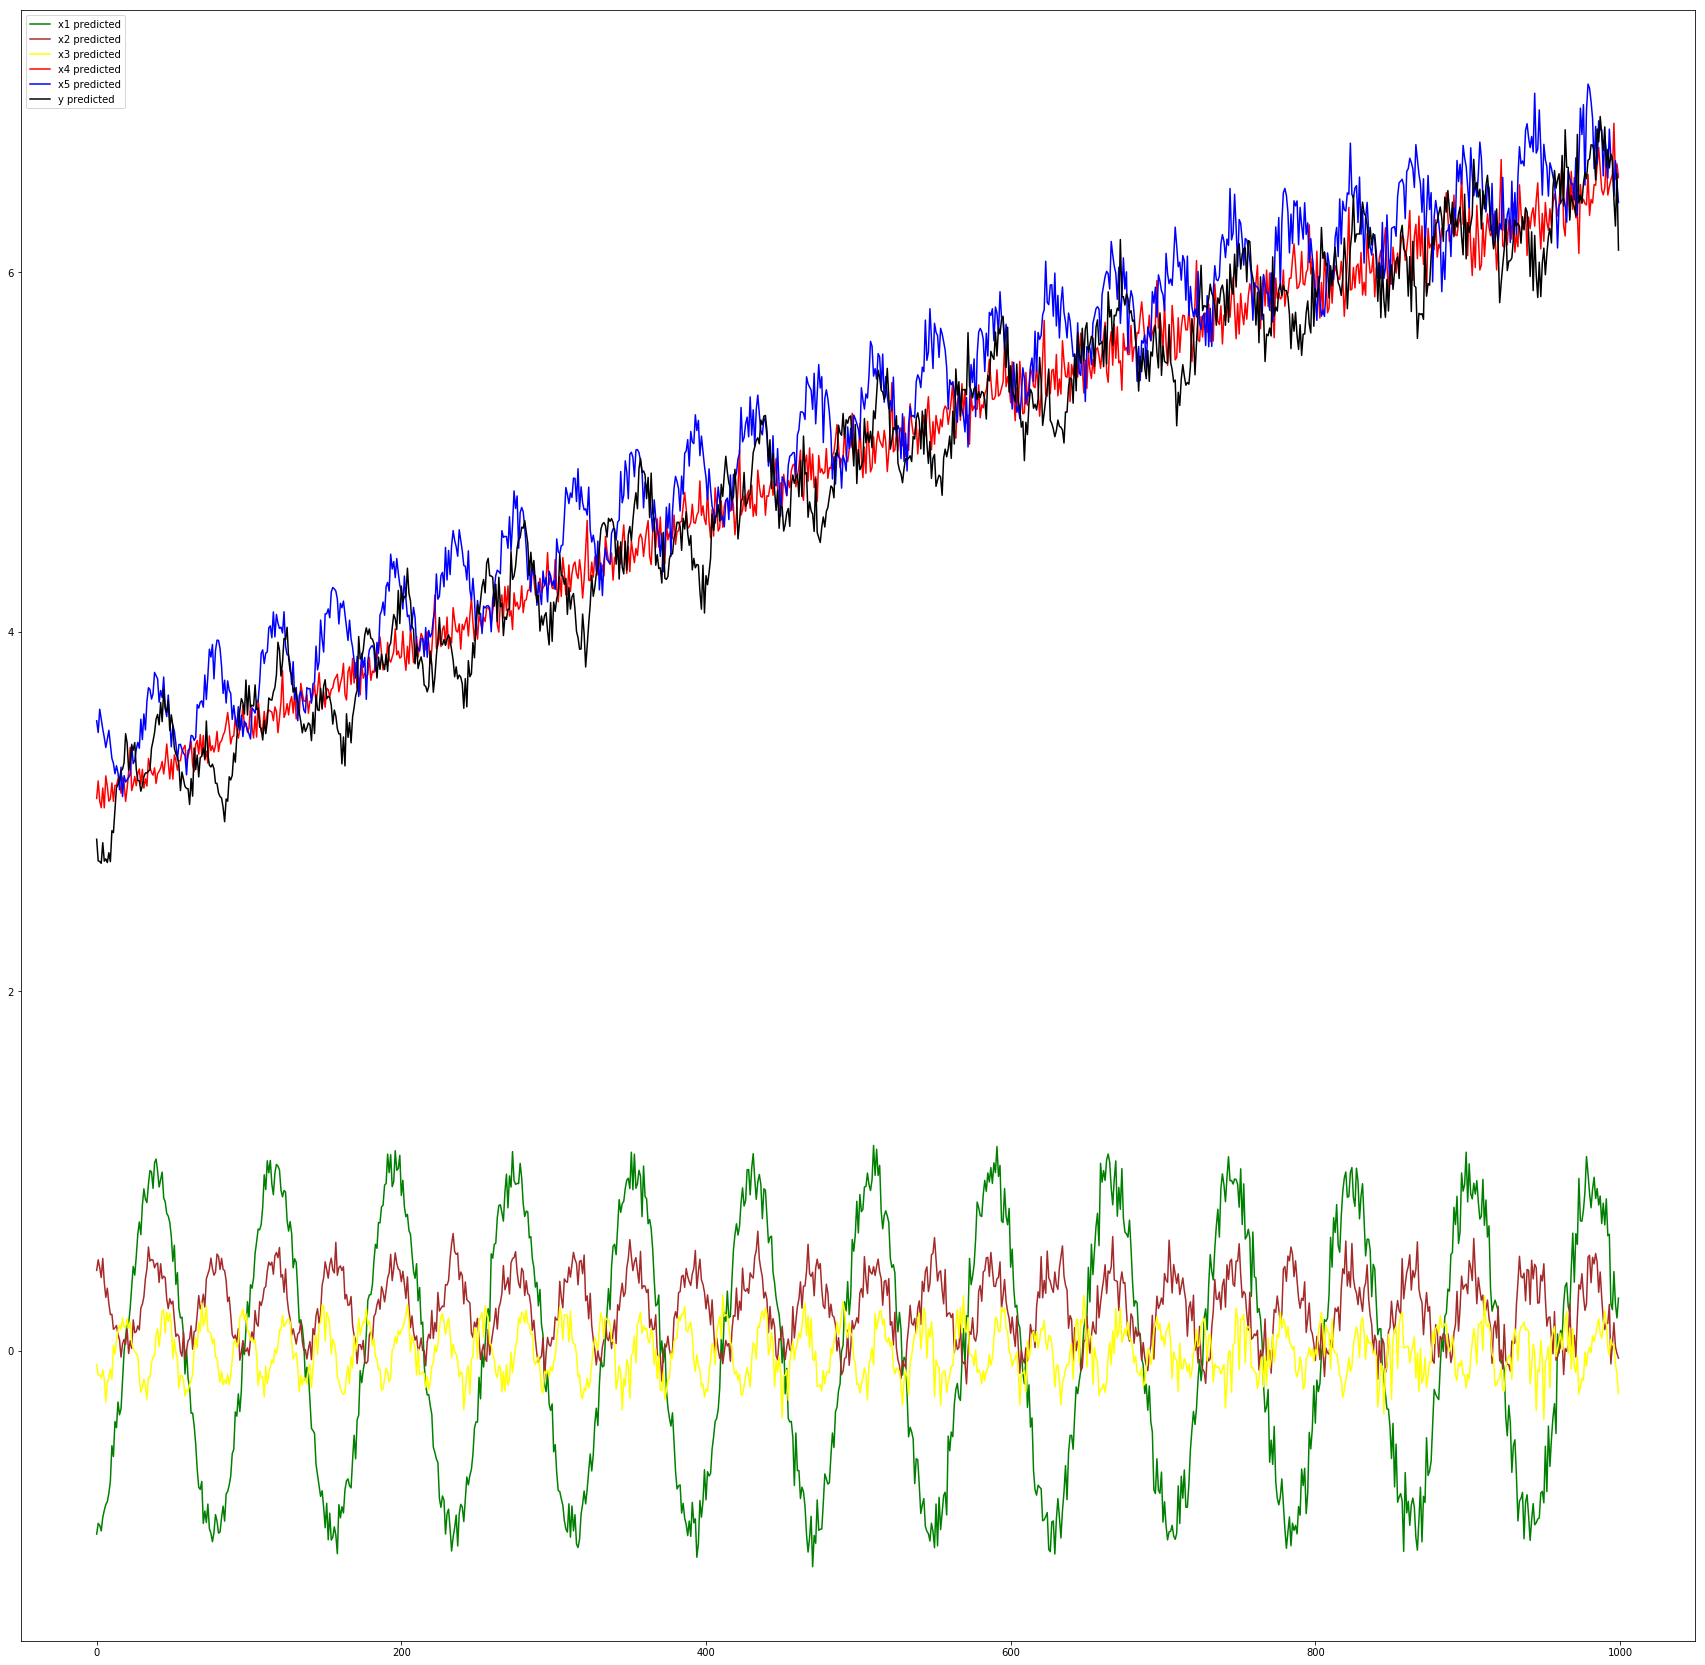
\includegraphics[width=0.9\textwidth]{./img/lstm_only_prediction.png}
% 	\caption{LSTM only model prediction}
% 	\label{img:lstm_only_prediction}
% \end{figure}

% \section{Влияние гиперпараметров модели на качество предсказаний}

% % todo
% % Посмотреть, как карта будет самобалансироваться, если сделать прикольную обратную связь.

% При уменьшении количества эпох обучения, карта может расходиться, даже карта с осмысленными связями.

% Увеличение параметра $ n\_steps\_in $, количество предыдущих значений временных рядов,
% а так же размерность скрытого состояния увеличивают количество требуемой для обучения
% памяти не более, чем линейно каждый. Конкретный показатель роста будет зависеть от
% плотности связей в карте.
% Уменьшение этих параметров, позволяет сэкономить память и ускорить обучение,
% но страдает качество предсказаний.


\section{Выводы}

В данной главе была реализована система для автоматического когнитивного картирования с использованием
методов нейронных сетей.
Также описаны инструменты, с помощью которых была реализована система.
Описана структура программного обеспечения, проведено тестирование разработанной системы.
На основе тестирования была дана оценка реализованной системе.

% Следует перечислить, какие практические результаты были получены, а именно: какое программное или иное обеспечение было создано. В число результатов могут входить, например, методики тестирования, тестовые примеры (для проверки корректности/оценки характеристик тех или иных алгоритмов) и др. По каждому результату следует сделать вывод, насколько он отличается от известных промышленных аналогов и исследовательских прототипов.



\clearpage

\chapter*{Заключение}
\addcontentsline{toc}{chapter}{Заключение}
% В заключении в тезисной форме необходимо отразить результаты работы:


В ходе работы были решены следующие задачи:

\begin{itemize}
	\item Разработан алгоритм для интеграции нейросетевых моделей с когнитвными картами;
	\item Сравнены разные модели предсказания временных рядов между собой;
	\item Спроектирована и реализована модель для когнитивного картирования с использованием
	авторегресионных и нейросетевых методов.
	\item Споректировано и реализовано веб-приложение для автоматического когнитивного картирования;
	\item Система протестирована;
\end{itemize}

% В будущем возможно использование гибридных нейро-нечетких систем не только для оптимизации
% нечетких когнитивных карт, но и для уменьшения вычислительных мощностей, требуемых для обучения
% нейросетей за счет использование некоторых экспертных знаний, которые должны отобразиться
% в топологии разрабатываемой нейросети.

% Хотя нейро-нечеткие система в виде TTR NFCM показала себя лучше классической НКК,
% для реализации данного метода все еще нужна работа эксперта: эксперт должен определить
% связи концептов. Хотя на небольших объемах данных это еще возможно, но при увеличении
% количества данных одному человеку их проанализировать становится слишком сложно.
% Поэтому в будущем можно сравнить исследованный метод с другими нейронными или
% статистическими методами для предсказания timeseries данных.

% Для этого также можно использовать XGBoost (бустинг деревьев решений), Long short-term memory (LSTM),
% Random Vector Functional-Link (RVFL), Vector Auto Regression (VAR).
% Плюсом таких методов является то, что при работе с ними, эксперту не требуется определять степень влияния
% одних концептов на другие.

% я не хочу строить карту!
% я хочу залить данные и получить результат
% в кк результат неявный
% и для настройки карты, подбора функции активации нужно
% много мароки

\clearpage

\nocite{*}

\phantomsection
%\addcontentsline{toc}{chapter}{\bibname}	% Добавляем список литературы в оглавление
\bibliography{chapters/biblio}		


% \phantomsection
% \addcontentsline{toc}{chapter}{\bibname}	% Добавляем список литературы в оглавление
% \bibliography{chapters/biblio}						% Подключаем BibTeX-базы

% =====================

%\addcontentsline{toc}{section}{Список литературы}
%\begin{thebibliography}{99}


%\bibitem{RCO1} {Ермаков А.Е.  Автоматизация онтологического инжиниринга в системах извлечения знаний из текста. М.: ООО ``ЭР СИ О'', Компьютерная лингвистика и интеллектуальные технологии: труды Международной конференци Диалог'2008, 2008.}


%\bibitem{Troel} {Троелсен Э. Язык программирования C\# 2008  и платформа .Net 3.5  М.: издательство <<Вильямс>>{}, 2010. 1344 с.}


%\bibitem{PBIRCH}{Ashwani Garg, Ashish Mangla, Neelima Gupta, Vasudha Bhatnagar PBIRCH: A scalable parallel clustering algorithm for incremental data. //Proceedings of 10th International Database Engineering and Applications Symposium IDEAS06, 2006}



%\end{thebibliography}


\clearpage

\appendix
\renewcommand{\appendixtocname}{Приложения}
\addappheadtotoc
\renewcommand{\chaptername}{Приложение}




% \begin{figure}
\chapter{Приложение 1. Результаты экспериментов}

\begin{table}%
    \caption{Значения коэффициентов параметров ARIMAX(2, 0, 3)x(0, 1, 1, 7) с экзогенными переменными: индикатор дня недели и индикатор Рождества}\label{tbl:cmp-1}
    \centering
    \begin{tabular}{|l|r||r|r|}
        \hline
            Параметр           &     Значение коэффициента  &  Дисперсия  &  P-value \\
        \hline
            intercept          &     3.7294                 &     1.686 &   0.027 \\
            Friday             &     0.0159                 &  2440.530 &   1.000 \\
            Monday             &     0.0045                 &  5202.932 &   1.000 \\
            Saturday           &    -0.0011                 &  7994.566 &   1.000 \\
            Sunday             &     0.0055                 &  4295.359 &   1.000 \\
            Thursday           &    -0.0069                 &  5951.614 &   1.000 \\
            Tuesday            &    -0.0007                 &  7381.431 &   1.000 \\
            Wednesday          &     0.0078                 &  3557.219 &   1.000 \\
            xmas               & -8738.4506                 &   399.352 &   0.000 \\
            ar.L1              &     0.0149                 &     0.067 &   0.824 \\
            ar.L2              &     0.8291                 &     0.056 &   0.000 \\
            ma.L1              &     0.3286                 &     0.074 &   0.000 \\
            ma.L2              &    -0.5438                 &     0.062 &   0.000 \\
            ma.L3              &    -0.1352                 &     0.038 &   0.000 \\
            ma.S.L7            &    -0.9363                 &     0.017 &   0.000 \\
            sigma2             &  1.264e+06                 &  3.87e+04 &   0.000 \\
        \hline
    \end{tabular}
    \label{tbl:arimax_coeffs_exogen}
\end{table}

% \end{figure}


% % \chapter{Основные правила форматирования}\label{app-format}

% %\addcontentsline{toc}{chapter}{}


% % Текст пояснительной записки должен готовиться для печати на листах формата А4, использоваться должен шрифт с засечками (Roman; обычно --- Times Roman или Times New Roman), 12 или 14 кегль. Размеры полей:

% % \begin{itemize}
% % 	\item верхнее: 20 мм.
% % 	\item нижнее: 20 мм.
% % 	\item левое: 10 мм.
% % 	\item правое: 25 мм.
% % \end{itemize}

% % Нумероваться должны все страницы, начиная с первой (титульной), однако сами номера следует проставлять на страницах, начиная со страницы реферата. Номер следует проставлять внизу страницу (в центре).

% % Заголовки оформляются тем же шрифтом, что и основной текст (т.е., соответственно, Times Roman или Times New Roman). Для заголовков первого уровня размер шрифта может быть больше размера шрифта основного текста (обычно 14-16).

% % Все разделы текста: реферат, оглавление, введение, три главы основного
% % содержания, список литературы, заключение, приложения --- должны снабжаться
% % содержательным заголовком и начинаться с новой страницы; сами заголовки следует
% % при этом центрировать (заголовки параграфов и пунктов выравниваются по ширине).
% % Следует обратить внимание, что заголовки всех разделов, кроме трех основных
% % глав, регламентированы; заголовки трех основных глав должны быть содержательными
% % и отражать суть соответствующей главы. Названия типа <<Аналитическая часть>> и <<Теоретическая глава>> --- \textit{недопустимы}.

% % Текст пояснительной записки может содержать рисунки и таблицы. Все рисунки и
% % таблицы должны снабжаться номерами и подписями:

% % \begin{itemize}

% % 	\item нумерация рисунков и таблиц должна быть сквозная (но раздельная, т.к. для рисунков своя, для таблиц --- своя);

% % 	\item в случае большого количества иллюстраций/таблиц, допускается <<вложенная>> нумерация (т.е. таблицу/рисунок можно снабжать составным номером в формате

% % 	$$\langle\mbox{номер главы}\rangle.\langle\mbox{номер внутри главы}\rangle;$$

% % 	\item подрисуночная подпись должна располагаться снизу по центру;

% % 	\item название таблицы следует помещать над таблицей слева, без абзацного
% % 	отступа в одну строку с ее номером через тире (ГОСТ 7.32-2001, п.6.6.1).

% % \end{itemize}

% % Здесь перечислены не все, а лишь основные требования к оформлению. Прочие
% % требования --- см. соответствующие ГОСТы.

% % Для того чтобы избежать больших отступов в списках, которые по умолчанию добавляют окружения \texttt{itemize} и \texttt{enumerate}, следует использовать
% % \texttt{compactitem} (для маркированных списков) и \texttt{compactenum} (для нумерованных списков) из пакета \texttt{paralist}.
% % Например:

% % \begin{compactitem}
% % 	\item это;
% % 	\item не нумерованный;
% % 	\item список;
% % 	\item без лишних промежутков.
% % \end{compactitem}

% % И для нумерованных списков:

% % \begin{compactenum}[1)]
% % 	\item нумерованные списки;
% % 	\item пакета \texttt{paralist};
% % 	\item еще и удобно настраивать;
% % 	\item (например, менять формат номера).
% % \end{compactenum}

% % \noindent или

% % \begin{compactenum}[a)]
% % 	\item это другой;
% % 	\item нумерованный;
% % 	\item список;
% % 	\item без лишних промежутков;
% % 	\item и с буквенной нумерацией.
% % \end{compactenum}

% % А если хочется нумерацию сделать ангоязычной, то нужно использовать окружение \texttt{other\-language} (таким образом: \verb|\begin{otherlanguage}[numerals=latin]{russian}|)

% % \setkeys{russian}{numerals=latin}
% % %\selectlanguage{russian}
% % %\begin{otherlanguage}[numerals=latin]{russian}
% % \begin{russian}
% % \begin{compactenum}[a)]
% % 	\item это другой;
% % 	\item нумерованный;
% % 	\item список;
% % 	\item без лишних промежутков;
% % 	\item и с буквенной нумерацией.
% % \end{compactenum}
% % \end{russian}
% % %\end{otherlanguage}

% % \textbf{Замечание.} По неизвестным причинам, переключения не происходит, хотя должно.

\clearpage

\chapter{Приложение 2. Отчет по тестированию разработанного модуля на Python}
\label{listing:test_report}

\begin{lstlisting}
    ============================== test session starts ===============================
    platform linux -- Python 3.7.6, pytest-5.3.5, py-1.8.1, pluggy-0.13.1 -- /home/d.tarasov/anaconda3/bin/python
    collected 6 items
    
    fcm_test.py::TestFcm::test_fit_on_history PASSED                           [ 16%]
    fcm_test.py::TestFcm::test_fit_on_history_with_exogen_param PASSED         [ 33%]
    fcm_test.py::TestFcm::test_sum_model PASSED                                [ 50%]
    fcm_test.py::TestFcm::test_double_freeze PASSED                            [ 66%]
    fcm_test.py::TestFcm::test_freeze_history_mismatch PASSED                  [ 83%]
    fcm_test.py::TestFcm::test_train_lstm PASSED                               [100%]
    
    =============================== 6 passed in 3.26s ================================
\end{lstlisting}



\clearpage

% 
% \chapter{Правила использования шаблона}\label{app-manual}

% Настоящий шаблон все еще несколько несовершенен в плане оформления: например, неправильная нумерация приложений, и еще несколько нюансов. В последующих версиях это будет исправляться.

% Ниже описана структура исходных текстов шаблона (и, соответственно, структура исходных текстов ПЗ).

% Головной файл --- \texttt{thesis-template.tex}. Его задача --- <<склеить>> вместе разные части ПЗ. Каждая часть (реферат, введение, каждая содержательная глава, заключение, библиография, приложения) выделяется в отдельный файл.

% \begin{itemize}
% 	\item[] \texttt{thesis-macro.tex} --- содержит определения различных макрокоманд, которые часто используются в конкретной работе, например, определения окружения для теорем, некоторые часто используемые формулы, и т.п.;
% 	\item[] \texttt{thesis-abstract.tex} --- содержит аннотацию;
% 	\item[] \texttt{thesis-intro.tex} --- содержит введение;
% 	\item[] \texttt{thesis-chapter1.tex} --- текст первой главы;
% 	\item[] \texttt{thesis-chapter2.tex} --- текст второй главы;
% 	\item[] \texttt{thesis-chapter3.tex} --- текст третьей главы;
% 	\item[] \texttt{thesis-bibl.tex} --- список литературы (только подключение к
% 	проекту);
% 	\item[] \texttt{biblio.bib} --- собственно библиография (в формате BibTeX);
% 	\item[] \texttt{thesis-conclusion.tex} --- заключение;
% 	\item[] \texttt{thesis-appendix1.tex} --- первое приложение;
% 	\item[] \texttt{thesis-appendix2.tex} --- второе приложение;
% \end{itemize}


% %Одна из первых вещей, которые необходимо сделать при использовании данного шаблона --- это отредактировать аргумент команды \verb|\headertext| в начале головного файла.

% Головной файл нужно менять лишь тогда, когда нужно добавить в проект новый файл, или удалить существующий (см. команду \verb|\input|). Обычно, это требуется, когда нужно добавить/удалить приложения.

% Для того, чтобы \LaTeX{} при компиляции автоматически <<подхватил>> задание, его нужно сохранить в формате pdf (например, с помощью вирутального принтера), поместить в ту же папку \texttt{/title} и назвать \texttt{task.pdf}. Точно также следует поступить с титульной страницей (\texttt{title.pdf}). При оформлении ПЗ для ВКР следует дополнительно поместить в папку \texttt{/title} pdf-версию листа с подписями, назвав файл \texttt{title-dep22.pdf}. После этого, нужно раскомментировать команду \verb|\includepdf[pages={-}, offset=0mm -0mm]{title/title-dep22.pdf}| в начале головного файла. Образцы и Word-шаблоны титульных листов для (РС)ПЗ к УИРам, НИРам, практикам и ВКР лежат в папках \texttt{/title/магистры} и \texttt{/title/бакалавры}.

% В этой версии шаблона используется BibTeX, поэтому для оформления списка
% литературы используются два файла: \texttt{thesis-bibl.tex} и
% \texttt{biblio.bib}. Использование BibTex дает ряд преимуществ. Не нужно
% заботиться о порядке сортировки, это делается автоматически; не нужно заботиться,
% на какие элементы библиографии есть ссылки --- печатаются только использованные в
% тексте элементы. Кроме того, многие курсовые проекты выполняются на протяжении ряда лет. С BibTex проще собирать список литературы и управлять им.

% \textbf{Замечание}. В шаблоне используется пакет \texttt{hyperref}, который делает две вещи: все перекрестные ссылки <<кликабельны>>, а также выделены (красной) рамочкой. Эти рамки \textit{не выводятся на печать}. Вместо цветных рамок, возможны другие способы выделения ссылок (см. документацию пакета).


\end{document}

